% -*- compile-command: "make slides.pdf" -*-
\documentclass{beamer} 
\usepackage{tikz}
\usepackage{amsmath,amssymb}
\usepackage{hyperref}
\usepackage{graphicx}

\usepackage[utf8]{inputenc}%for french accents. 
%\usepackage{appendixnumberbeamer}

\addtobeamertemplate{navigation symbols}{}{%
    \usebeamerfont{footline}%
    \usebeamercolor[fg]{footline}%
    \hspace{1em}%
    \insertframenumber/\inserttotalframenumber
}

\DeclareMathOperator*{\argmin}{arg\,min}
\DeclareMathOperator*{\Lik}{Lik}
\DeclareMathOperator*{\Peaks}{Peaks}
\DeclareMathOperator*{\Segments}{Segments}
\DeclareMathOperator*{\argmax}{arg\,max}
\DeclareMathOperator*{\maximize}{maximize}
\DeclareMathOperator*{\minimize}{minimize}
\newcommand{\sign}{\operatorname{sign}}
\newcommand{\RR}{\mathbb R}
\newcommand{\ZZ}{\mathbb Z}
\newcommand{\NN}{\mathbb N}
\definecolor{pDPA}{HTML}{1B9E77}
\definecolor{PELT}{HTML}{D95F02}
\definecolor{FPOP}{HTML}{7570B3}
\newcommand{\algo}[1]{\textcolor{#1}{#1}}
\definecolor{PDPA}{HTML}{66C2A5}
\definecolor{CDPA}{HTML}{FC8D62}
\definecolor{GPDPA}{HTML}{4D4D4D}




% Set transparency of non-highlighted sections in the table of
% contents slide.
\setbeamertemplate{section in toc shaded}[default][100]
\AtBeginSection[]
{
  \setbeamercolor{section in toc}{fg=red} 
  \setbeamercolor{section in toc shaded}{fg=black} 
  \begin{frame}
    \tableofcontents[currentsection]
  \end{frame}
}

\begin{document}

\title{Same vs. other cross-validation in supervsied machine learning}
\author{
  Toby Dylan Hocking\\
  toby.hocking@nau.edu
}

\maketitle

\section{Introduction to machine learning}

\begin{frame}
  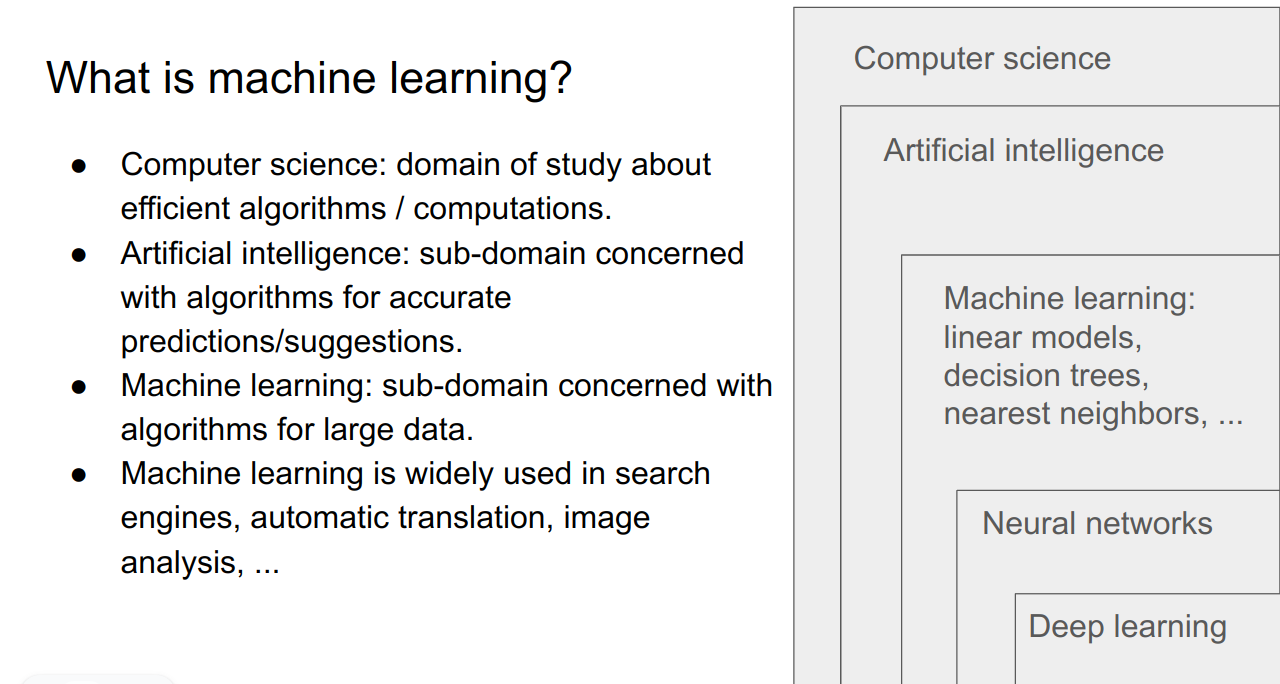
\includegraphics[width=\textwidth]{figure-ai-vs-ml}
\end{frame}

\begin{frame}
  \frametitle{Machine learning intro: image classification example}
  ML is all about learning predictive functions $f(x)\approx y$, where 
  \begin{itemize}
  \item Inputs/features $x$ can be easily computed using traditional
    algorithms, e.g. matrix of pixel intensities in an image.
  \item Outputs/labels $y$ are what we want to predict, easy to get by
    asking a human, but hard to compute using traditional algorithms,
    e.g. image class.
  \item Input $x$ = image of digit, output $y\in\{0,1,\dots,9\}$, \\--
    this is a classification problem with 10 classes.\\
  $f(
\includegraphics[height=1cm]{mnist-0})=0$,
  $f(
\includegraphics[height=1cm]{mnist-1})=1$
\item Traditional/unsupervised algorithm: I give you a pixel intensity matrix
  $x\in\RR^{16\times 16}$, you code a function $f$ that returns one of
  the 10 possible digits. Q: how to do that?
  \end{itemize}
\end{frame}

\begin{frame}
  \frametitle{Supervised machine learning algorithms}

  I give you a training data set with paired inputs/outputs, e.g.

  \begin{center}
    \Huge $y=$\ 0 1 2 3 4 5 6 7 8 9

$X=$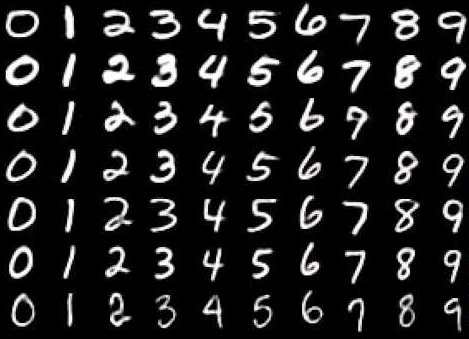
\includegraphics[height=1.9in]{mnist-digits}
  \end{center}

  Your job is to code an algorithm that learns the function $f$ from
  the training data. (you don't code $f$)
  
  \scriptsize Source: github.com/cazala/mnist
\end{frame}

\begin{frame}
  \frametitle{Supervised machine learning algorithms}

  \textbf{Can} be used whenever a knowledgeable/skilled
  human can easily/quickly/consistently create a large database of
  labels for training.

  \vskip 1cm

  \textbf{Should} be used if it is not easy to code the function $f$
  for predicting the labels (using traditional/unsupervised
  techniques).

  \vskip 1cm

  \textbf{Accurate} if the test data, on which you want to use $f$, is
  similar to the train data (input to learning algorithm).

\end{frame}



\begin{frame}
  \frametitle{Advantages of supervised machine learning}

  \begin{center}
      \begin{tabular}{cc}
        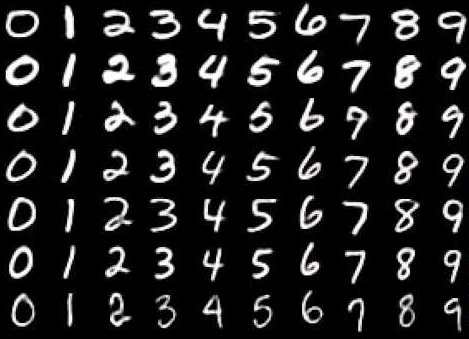
\includegraphics[height=1.5in]{mnist-digits} &
  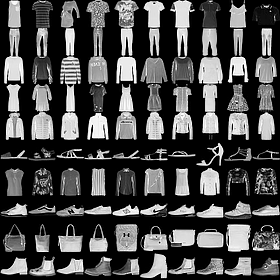
\includegraphics[height=1.5in]{fashion-mnist-sprite-some}  
  \end{tabular}
  \end{center}
  \vskip -0.2cm
  
  \begin{itemize}
  \item Input $x\in\RR^{16\times 16}$, output $y\in\{0,1,\dots,9\}$ types the same!
  \item Can use same learning algorithm regardless of pattern.
  \item Pattern encoded in the labels (not the algorithm).
  \item Useful if there are many un-labeled data, but few labeled data
    (or getting labels is long/costly).
  \item State-of-the-art accuracy (if there is enough training data).
  \end{itemize}

  \scriptsize Sources: github.com/cazala/mnist, github.com/zalandoresearch/fashion-mnist

\end{frame}


\begin{frame}
  \frametitle{Learning two different functions using two data sets} Figure from chapter by Hocking TD,
  \textit{Introduction to machine learning and neural networks} for
  book \textit{Land Carbon Cycle Modeling: Matrix Approach, Data
    Assimilation, and Ecological Forecasting} edited by Luo Y (Taylor
  and Francis, 2022).
  \begin{center}
  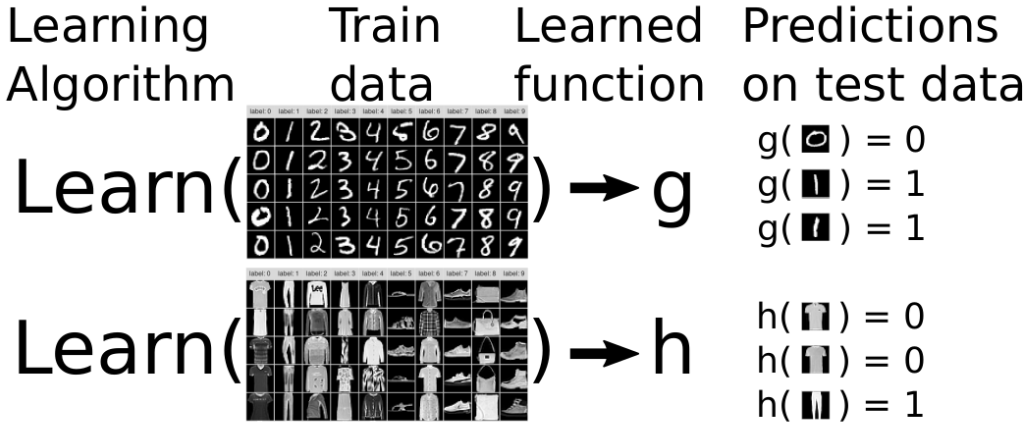
\includegraphics[width=\textwidth]{figure-learn-digits-clothing}
\end{center}
  \textbf{Learn} is a learning algorithm, which outputs
  $g$ and $h$.

  Q: what happens if you do
    $g(
\includegraphics[height=1cm]{fashion-mnist-boot})$, or
    $h(
\includegraphics[height=1cm]{mnist-0})$?
\end{frame}

\begin{frame}
  \frametitle{Learning two different functions using two data sets} 
  \begin{itemize}
  \item What if you do
    $g(
\includegraphics[height=1cm]{fashion-mnist-boot})$, or
    $h(
\includegraphics[height=1cm]{mnist-0})$?
  \item This is a question about \textbf{generalization}: how accurate is the
    learned function on a new/test data set?
  \item ``Very accurate'' if test data are similar enough to train data (best case is i.i.d. = independent and identically distributed)
  \item Predicting childhood autism (Lindly \emph{et al.}), train on
    one year of surveys, test on another.
  \item Predicting carbon emissions (Aslam \emph{et al.}), train on
    one city, test on another.
  \item Predicting presence of trees/fires in satellite imagery
    (Shenkin \emph{et al.}, \emph{Thibault} \emph{et al.}), train on
    one geographic area/image, test on another.
  \item Predicting fish spawning habitat in sonar imagery (Bodine
    \emph{et al.}), train on one river, test on another.
  \item But how do we check if ``very accurate'' in these situations?
  \end{itemize}
\end{frame}

\section{Proposed same vs. other cross-validation}

\begin{frame}
  \frametitle{$K$-fold cross-validation: a standard algorithm used to estimate the prediction accuracy in machine learning}

  \begin{itemize}
  \item $K=3$ folds shown in figure below, meaning three different
    models trained, and three different prediction/test accuracy rates
    computed.
  \item It is important to use several train/test splits, so we can
    see if there are statistically significant differences between
    algorithms.
  \end{itemize}

  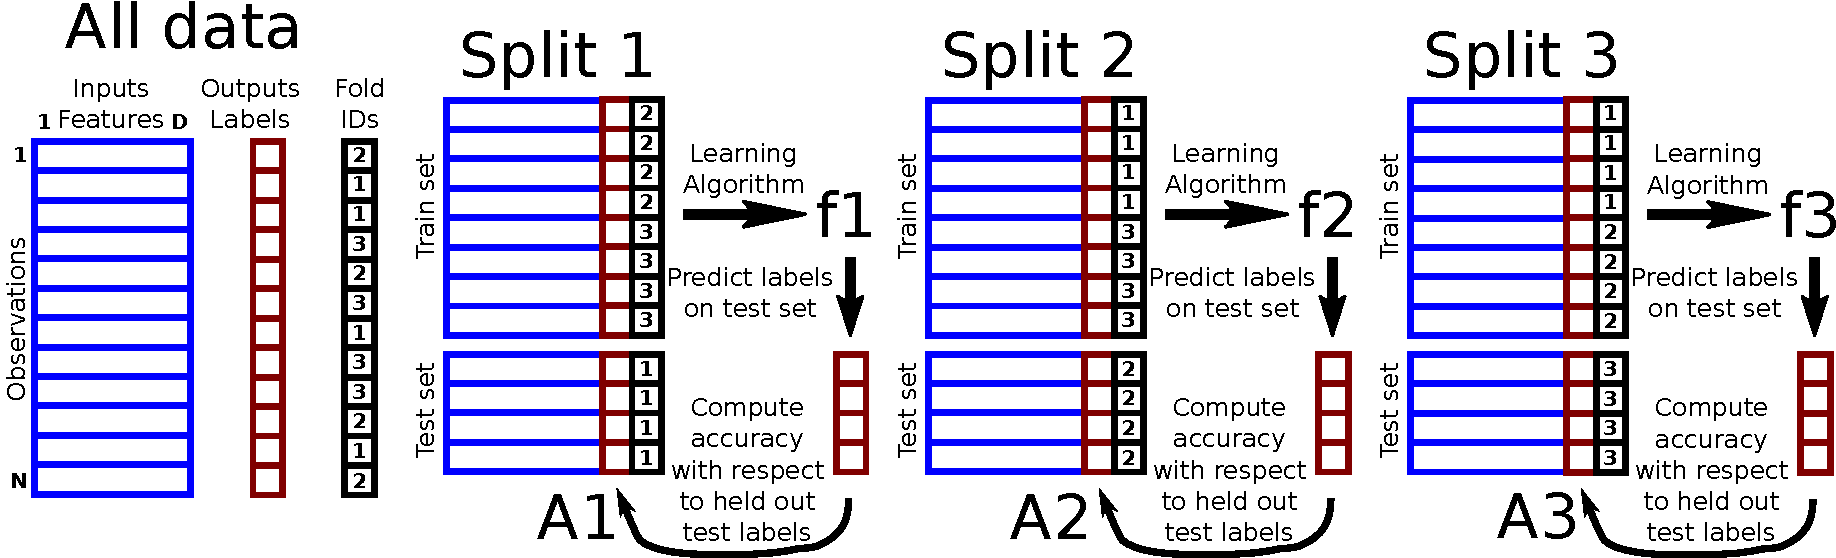
\includegraphics[width=\textwidth]{drawing-cross-validation.pdf}

  \small Hocking TD \emph{Intro. to machine learning and neural
    networks} (2022).
\end{frame}

\begin{frame}
  \frametitle{Example data set: predicting childhood autism}

  \begin{itemize}
  \item Collaboration with Lindly \emph{et al.}
  \item Downloaded National Survey of Children's Health (NSCH) data,
    years 2019 and 2020, from
    \url{http://www2.census.gov/programs-surveys/nsch}
  \item One row per person, one column per survey question.
  \item Pre-processing to obtain common columns over the two years,
    remove missing values, one-hot/dummy variable encoding.
  \item Result is $N=46,010$ rows and $D=366$ columns.
  \item 18,202 rows for 2019; 27,808 rows for 2020.
  \item One column is diagnosis with Autism (binary
    classification, yes or no), can we predict it using the others?
  \item Can we combine data from different years?
  \item Can we train on one year, and accurately predict on another?
  \end{itemize}

\end{frame} 


\begin{frame}
  \frametitle{Proposed Same Other Cross-Validation}
  \begin{itemize}
  \item Example: childhood autism prediction data set.
  \end{itemize}
  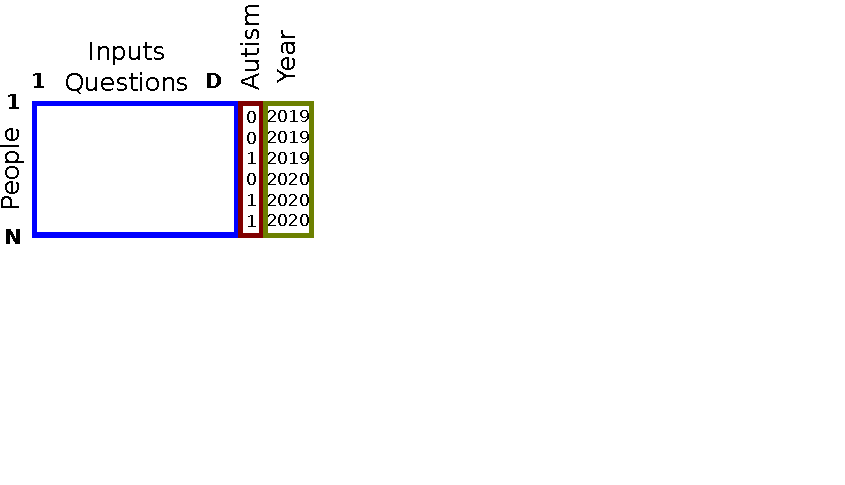
\includegraphics[width=\textwidth]{drawing-cv-same-other-years-1.pdf}
\end{frame}

\begin{frame}
  \frametitle{Proposed Same Other Cross-Validation}
  \begin{itemize}
  \item Train group same as test (=regular $K$-fold CV on 2020).
  \end{itemize}
  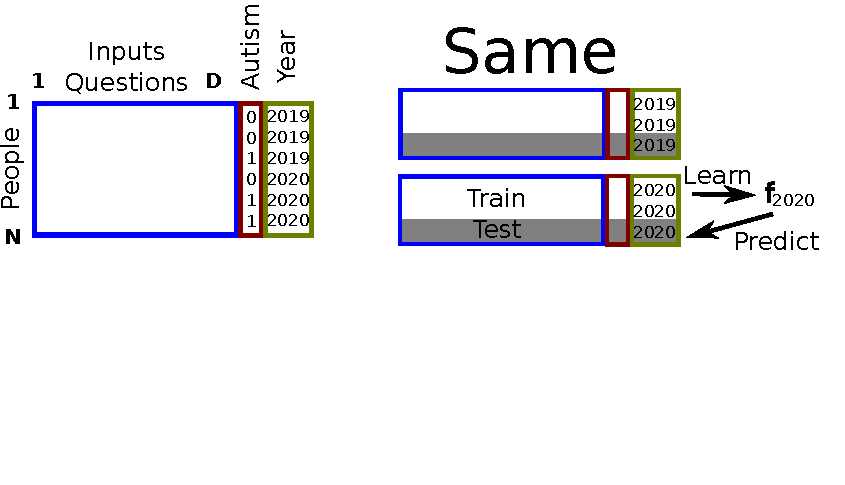
\includegraphics[width=\textwidth]{drawing-cv-same-other-years-2.pdf}
\end{frame}

\begin{frame}
  \frametitle{Proposed Same Other Cross-Validation}
  \begin{itemize}
  \item Train group (2019) different from test (2020).
  \end{itemize}
  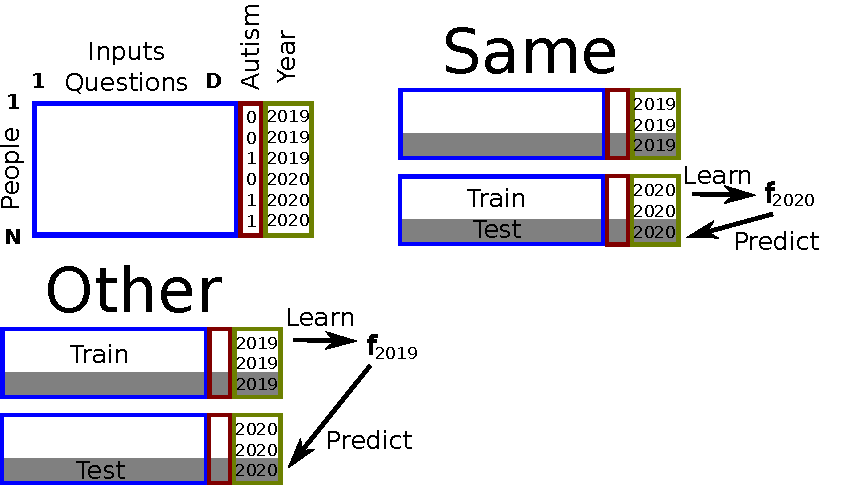
\includegraphics[width=\textwidth]{drawing-cv-same-other-years-3.pdf}
\end{frame}

\begin{frame}
  \frametitle{Proposed Same Other Cross-Validation}
  \begin{itemize}
  \item Repeat for each of $K$ folds, and each test group (2019,2020).
  \end{itemize}
  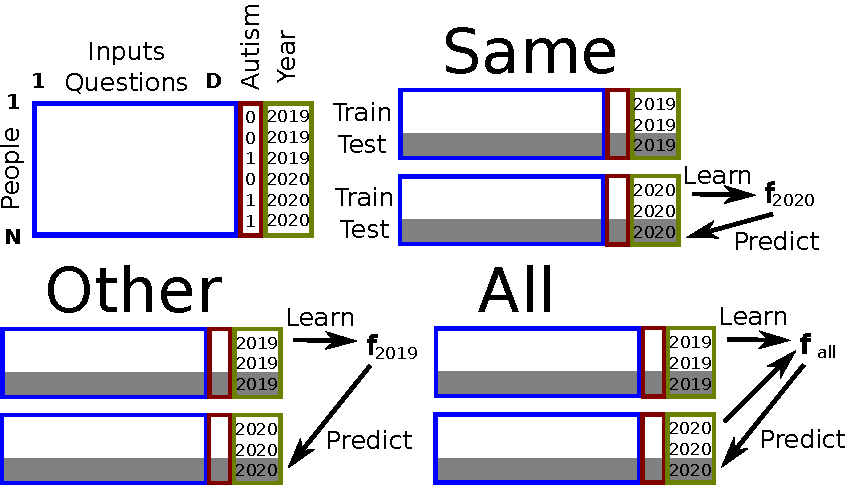
\includegraphics[width=\textwidth]{drawing-cv-same-other-years-4.pdf}
\end{frame}

\begin{frame}
  \frametitle{Proposed Same Other Cross-Validation}
  For a fixed test set from one group:
  
  If train/test are similar/iid,
  \begin{description}
  \item[All] should be most accurate.
  \item[Same/Other] should be less accurate, because there is less
    data available (if other is larger than same, then other should be
    more accurate than same, etc).
  \end{description}

  If train/test are different (not iid),
  \begin{description}
  \item[Same] should be most accurate.
  \item[Other] should be substantially less accurate.
  \item[All] accuracy should be between same and other.
  \end{description}
\end{frame}

\section{Results on real data sets}

\begin{frame}
  \frametitle{Learning algorithms we consider}
  We used the following learning algorithms:
\begin{description}
\item[cv\_glmnet] L1-regularized linear model (feature
  selection). Friedman, \emph{et al.} (2010).
  % Friedman J, Tibshirani R, Hastie T (2010). “Regularization Paths for
  % Generalized Linear Models via Coordinate Descent.” _Journal of
  % Statistical Software_, *33*(1), 1-22. doi:10.18637/jss.v033.i01
  % <https://doi.org/10.18637/jss.v033.i01>.
\item[xgboost] Extreme gradient boosting (non-linear). Chen and Guestrin (2016). 
\item[rpart] Recursive partitioning, decision tree (non-linear, feature selection). Therneau and Atkinson (2023).
  % Therneau T, Atkinson B (2023). _rpart: Recursive Partitioning and
  % Regression Trees_. R package version 4.1.23,
  % <https://CRAN.R-project.org/package=rpart>.
\item[nearest\_neighbors] classic non-linear algorithm, as implemented
  in kknn R package. Schliep and Hechenbichler (2016).
  % Schliep K, Hechenbichler K (2016). _kknn: Weighted k-Nearest
  % Neighbors_. R package version 1.3.1,
  % <https://CRAN.R-project.org/package=kknn>.
\item[featureless] un-informed baseline, ignores all inputs/features,
  and always predicts the most frequent label in train data. For
  example, Autism=No. Nomenclature from mlr3 R package,
  Lang, \emph{et al.}, (2019).
  % Lang M, Binder M, Richter J, Schratz P, Pfisterer F, Coors S, Au Q,
  % Casalicchio G, Kotthoff L, Bischl B (2019). “mlr3: A modern
  % object-oriented machine learning framework in R.” _Journal of Open
  % Source Software_. doi:10.21105/joss.01903
  % <https://doi.org/10.21105/joss.01903>,
  % <https://joss.theoj.org/papers/10.21105/joss.01903>.
\end{description}
Each learning algorithm has different properties (non-linear, feature
selection, etc). For details see Hastie, {\it et al.} (2009) textbook.
\end{frame}

\begin{frame}
  \frametitle{$K$-fold CV on NSCH data (predict autism), year 2020}
  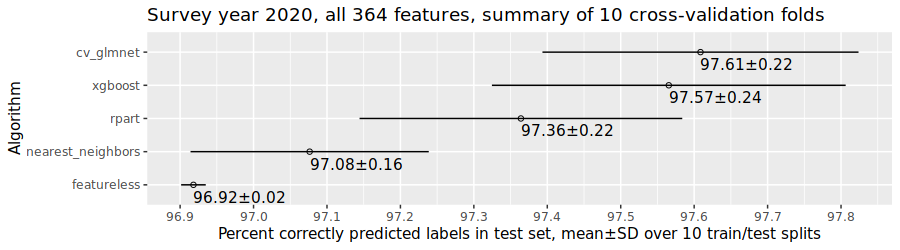
\includegraphics[width=\textwidth]{download-nsch-mlr3batchmark-registry-one-set-all-features-stats.png}

Learning algorithms we consider:
\begin{description}
\item[cv\_glmnet] L1-regularized linear model (feature selection).
\item[xgboost] Extreme gradient boosting (non-linear).
\item[rpart] Recursive partitioning, decision tree (non-linear, feature selection).
\item[nearest\_neighbors] classic non-linear algorithm.
\item[featureless] un-informed baseline, ignores all inputs/features,
  and always predicts the most frequent label in train data (Autism=No
  in this case).
\end{description}

\end{frame}

\begin{frame}
  \frametitle{Same Other CV for Autism data}
  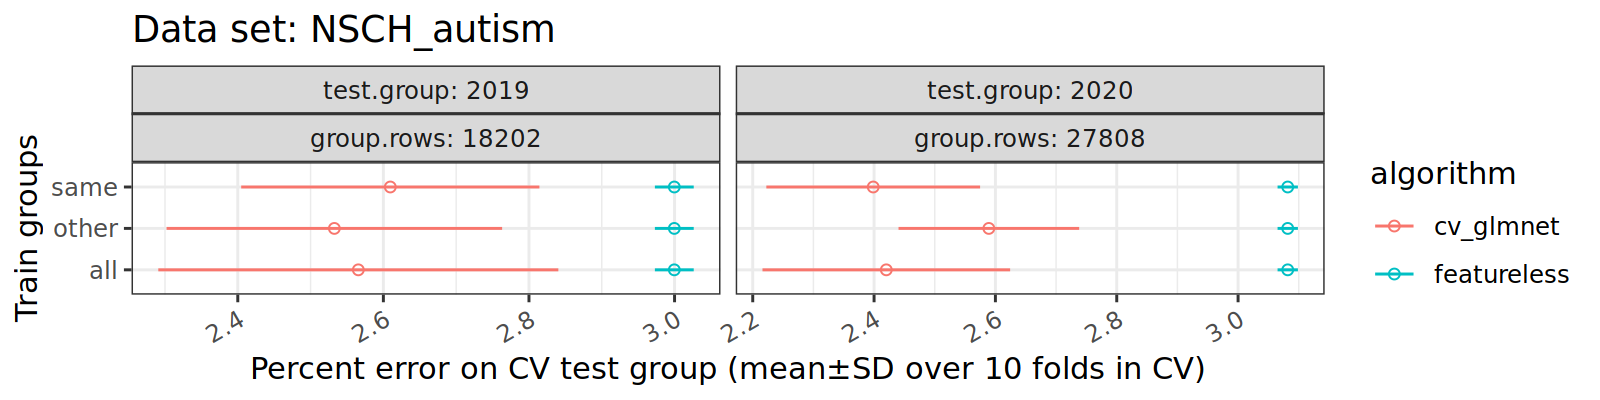
\includegraphics[width=\textwidth]{NSCH_autism_error_glmnet_featureless_mean_SD.png}
  \begin{itemize}
  \item Each cv\_glmnet model has significantly less error than
    featureless, indicating that some non-trivial pattern has been
    learned.
  \end{itemize}
\end{frame}

\begin{frame}
  \frametitle{Same Other CV for Autism data}
  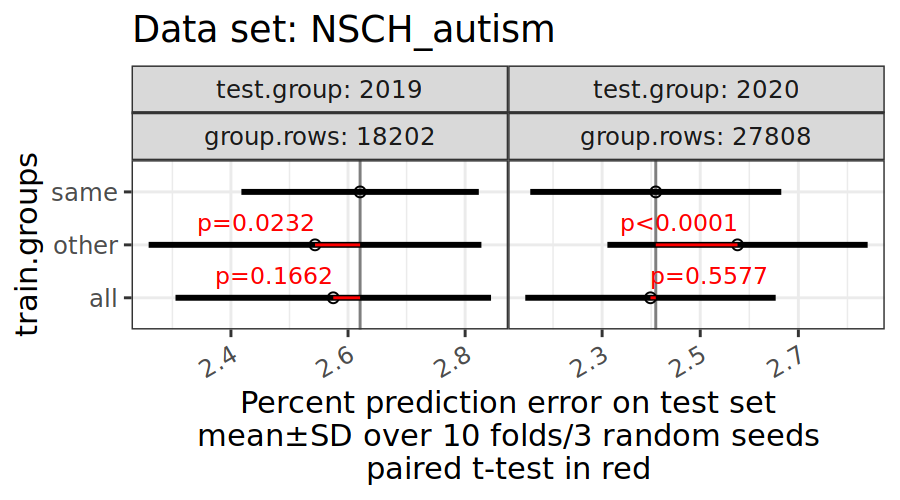
\includegraphics[width=\textwidth]{NSCH_autism_error_glmnet_sizes_mean_SD_pvalue.png}
  
  \vskip -0.4cm
  
  \begin{itemize}
  \item All has slightly less error than same, which suggests the
    two years have similar patterns, and can be combined for learning
    a more accurate model.
  \item Other has either less error or more, suggesting that the error
    rate depends on the number of rows in the train set.
  \end{itemize}
\end{frame}

\begin{frame}
  \frametitle{Example data 2: Canada fires}
% > meta.dt[data.name=="CanadaFires_all"]
%          data.name memory.kb  rows n.groups                         group.tab
%             <char>     <int> <int>    <int>                            <char>
% 1: CanadaFires_all      1122  4827        4 306=364;329=755;395=1170;326=2538
%    group.small.name group.small.N group.large.name group.large.N
%              <char>         <int>           <char>         <int>
% 1:              306           364              326          2538
%    label.small.name label.small.N label.large.name label.large.N features
%              <char>         <int>           <char>         <int>    <int>
% 1:           burned          1629          no burn          3198       46
%    classes min.rows  test train test%
%      <int>    <int> <int> <int> <int>
% 1:       2      140    NA    NA    NA  
  \begin{itemize}
  \item Collaboration with Thibault \emph{et al.}
  \item Satellite image data, $N=4827$ rows/pixels, $D=46$
    features/spectral bands.
  \item Government land management project: oal is to predict whether
    the pixel has been burned (binary classification, yes or no).
  \item Four satellite images in different regions of the forest,
    numbered 306, 326, 329, 395.
  \item Can we train on one image, and accurately predict on another?
  \end{itemize}
\end{frame}

\begin{frame}
  \frametitle{Same Other CV for Canada fires data}
  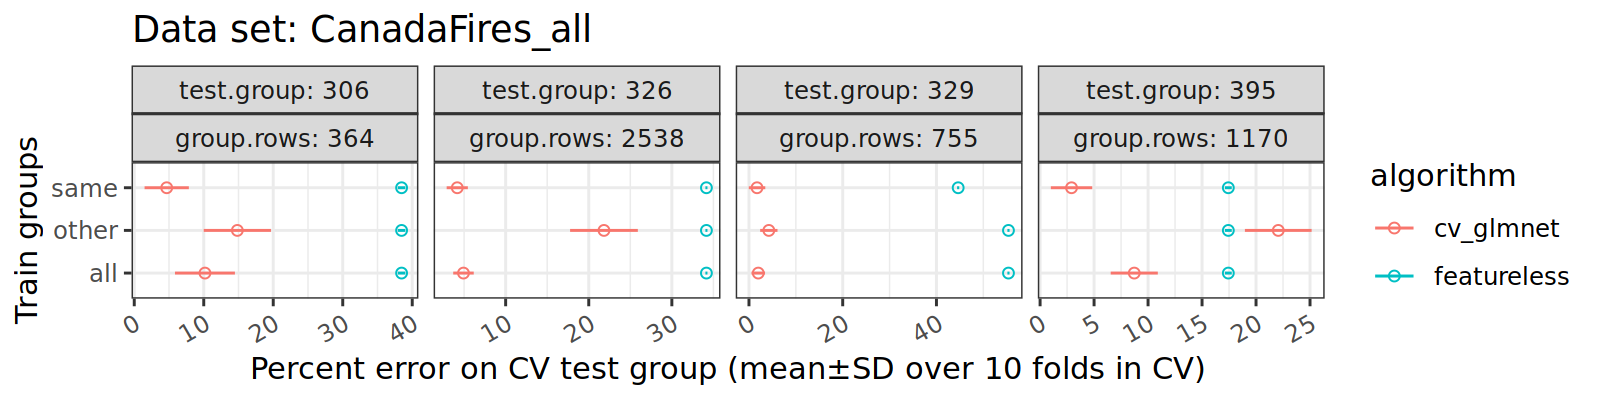
\includegraphics[width=\textwidth]{CanadaFires_all_error_glmnet_featureless_mean_SD.png}
  \begin{itemize}
  \item Each cv\_glmnet model has significantly less error than
    featureless, except train.groups=other for test.group=395 (must
    have a very different pattern than the other images).
  \item Training on all images is never as accurate as same, which
    suggests that images are substantially different, and we need
    labels from the same image to get optimal predictions.
  \end{itemize}
\end{frame}

\begin{frame}
  \frametitle{Example data 3: AZ trees}
% > meta.dt[data.name=="aztrees3"]
%    data.name memory.kb  rows n.groups              group.tab group.small.name
%       <char>     <int> <int>    <int>                 <char>           <char>
% 1:  aztrees3       587  5956        3 NE=1464;NW=1563;S=2929               NE
%    group.small.N group.large.name group.large.N label.small.name label.small.N
%            <int>           <char>         <int>           <char>         <int>
% 1:          1464                S          2929         Not tree          5282
%    label.large.name label.large.N features classes min.rows  test train test%
%              <char>         <int>    <int>   <int>    <int> <int> <int> <int>
% 1:             Tree           674       21       2       55    NA    NA    NA
  \begin{itemize}
  \item Collaboration with Shenkin \emph{et al.}
  \item Satellite image data, $N=5956$ rows/pixels, $D=21$
    features/spectral bands.
  \item Tree stress project: goal is to predict whether the pixel has
    a tree (binary classification, yes or no).
  \item Three regions around Flagstaff: NE, NW, S.
  \item Can we train in one region, and accurately predict on another?
  \end{itemize}
\end{frame}

\begin{frame}
  \frametitle{Same Other CV for AZ trees data}
  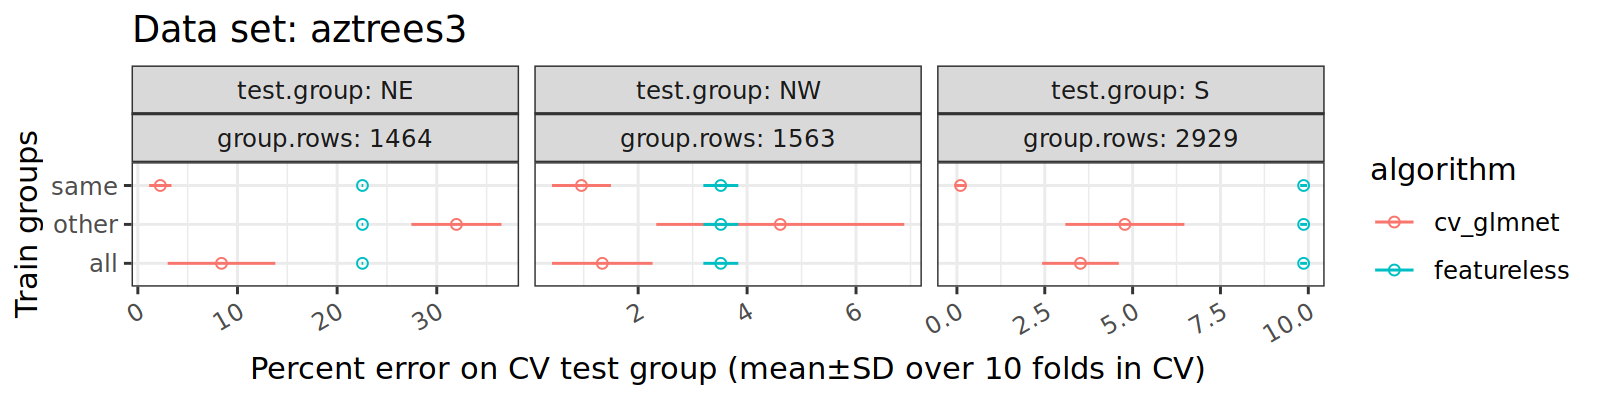
\includegraphics[width=\textwidth]{aztrees3_error_glmnet_featureless_mean_SD.png}
  \begin{itemize}
  \item Each cv\_glmnet model has significantly less error than
    featureless, except train.groups=other for two test groups (must
    have a very different pattern than the other images).
  \item Training on all images is never as accurate as same, which
    suggests that images are substantially different, and we need
    labels from the same image to get optimal predictions.
  \end{itemize}
\end{frame}

\begin{frame}
  \frametitle{Example data 4: fish sonar}
% > meta.dt[data.name=="FishSonar_river"]
%          data.name memory.kb    rows n.groups
%             <char>     <int>   <int>    <int>
% 1: FishSonar_river    934937 2815744        4
%                                      group.tab group.small.name group.small.N
%                                         <char>           <char>         <int>
% 1: CHI=638475;PRL=667201;LEA=739745;BOU=770323              CHI        638475
%    group.large.name group.large.N label.small.name label.small.N
%              <char>         <int>           <char>         <int>
% 1:              BOU        770323             hard        677258
%    label.large.name label.large.N features classes min.rows  test train test%
%              <char>         <int>    <int>   <int>    <int> <int> <int> <int>
% 1:            other       2138486       81       2   113592    NA    NA    NA
  \begin{itemize}
  \item Collaboration with Bodine \emph{et al.}
  \item Sonar image data, $N=2,815,744$ rows/pixels, $D=81$
    features (mean pixel intesity in windows around target pixel).
  \item Conservation project funded by Department of Fish/Wildlife:
    goal is to predict whether the pixel has a hard bottom suitable
    for fish spawning (binary classification, yes or no).
  \item Four rivers in southeast USA: CHI, PRL, LEA, BOU.
  \item Can we train in one river, and accurately predict on another?
  \end{itemize}
\end{frame}

\begin{frame}[fragile]
  \frametitle{Same Other CV for fish sonar data}
  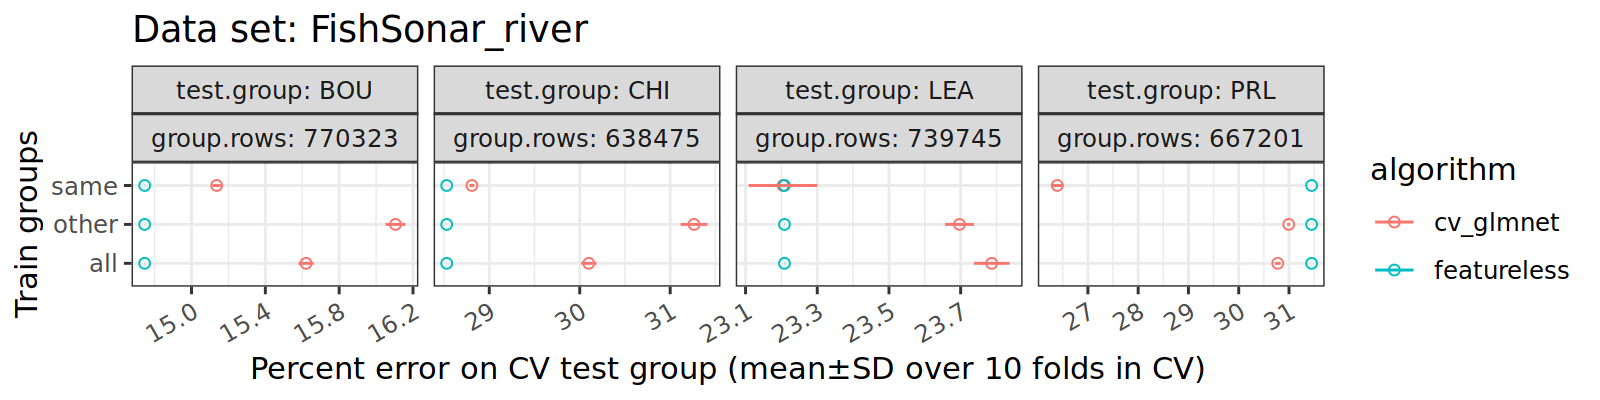
\includegraphics[width=\textwidth]{FishSonar_river_error_glmnet_featureless_mean_SD.png}
  \begin{itemize}
  \item When training on same group, cv\_glmnet sometimes has larger
    test error than featureless, because of class imbalance (hard
    bottom suitable for fish spawning is rare).
  \end{itemize}
\begin{verbatim}
       river
label      BOU    CHI    LEA    PRL
  hard  113592 182150 171684 209832
  other 656731 456325 568061 457369
\end{verbatim}
\end{frame}

\begin{frame}
  \frametitle{Same Other CV for fish sonar data}
  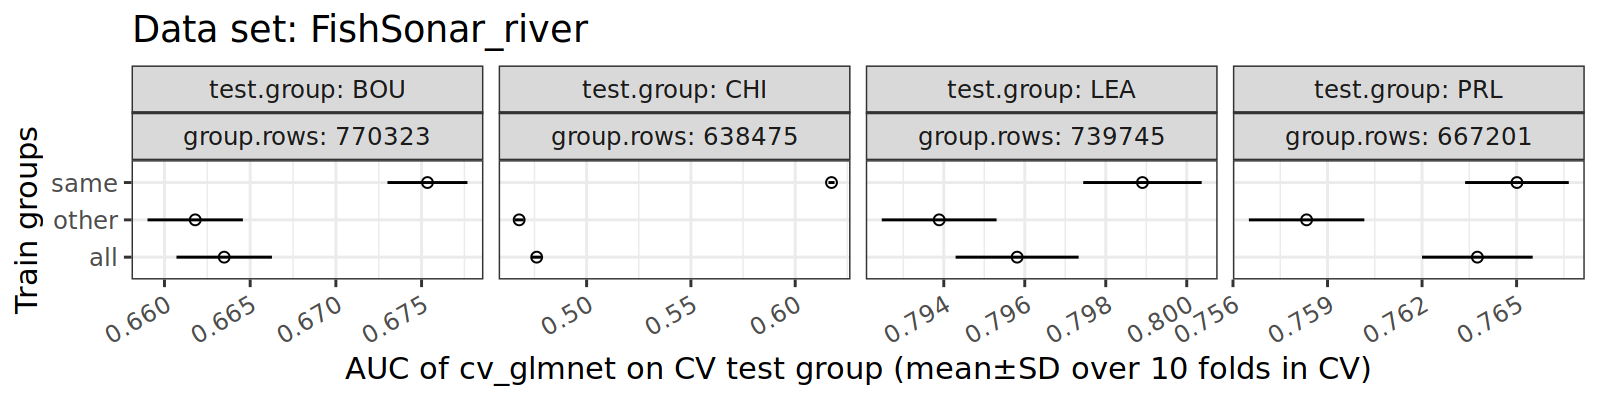
\includegraphics[width=\textwidth]{FishSonar_river_AUC_glmnet_mean_SD.png}
  \begin{itemize}
  \item Area Under the ROC Curve (AUC) is a good measure of accuracy
    for imbalanced binary classification problems (constant/featureless=0.5, best=1).
  \item Mostly test AUC is greater than 0.5, which means a non-trivial
    prediction function has been learned.
  \item For test.group=CHI with train.groups=all/other, test
    AUC$<0.5$, indicating a very different pattern in this river
    (opposite of the pattern in other rivers).
  \item Test AUC for all is never as large as same, indicating that
    you need data from the same river for optimal prediction accuracy.
  \end{itemize}
\end{frame}

\section{Results on machine learning benchmark data sets}

\begin{frame}
  \frametitle{Train on MNIST and accurately predict on EMNIST?}

  Recall: what happens if you do
  $g(
\includegraphics[height=1cm]{fashion-mnist-boot})$, or
  $h(
\includegraphics[height=1cm]{mnist-0})$?
  
  \begin{itemize}
  \item Boot image comes from FashionMNIST data, which were used to learn $h$.
  \item 0 image comes from MNIST data, which were used to learn $g$.
  \end{itemize}

  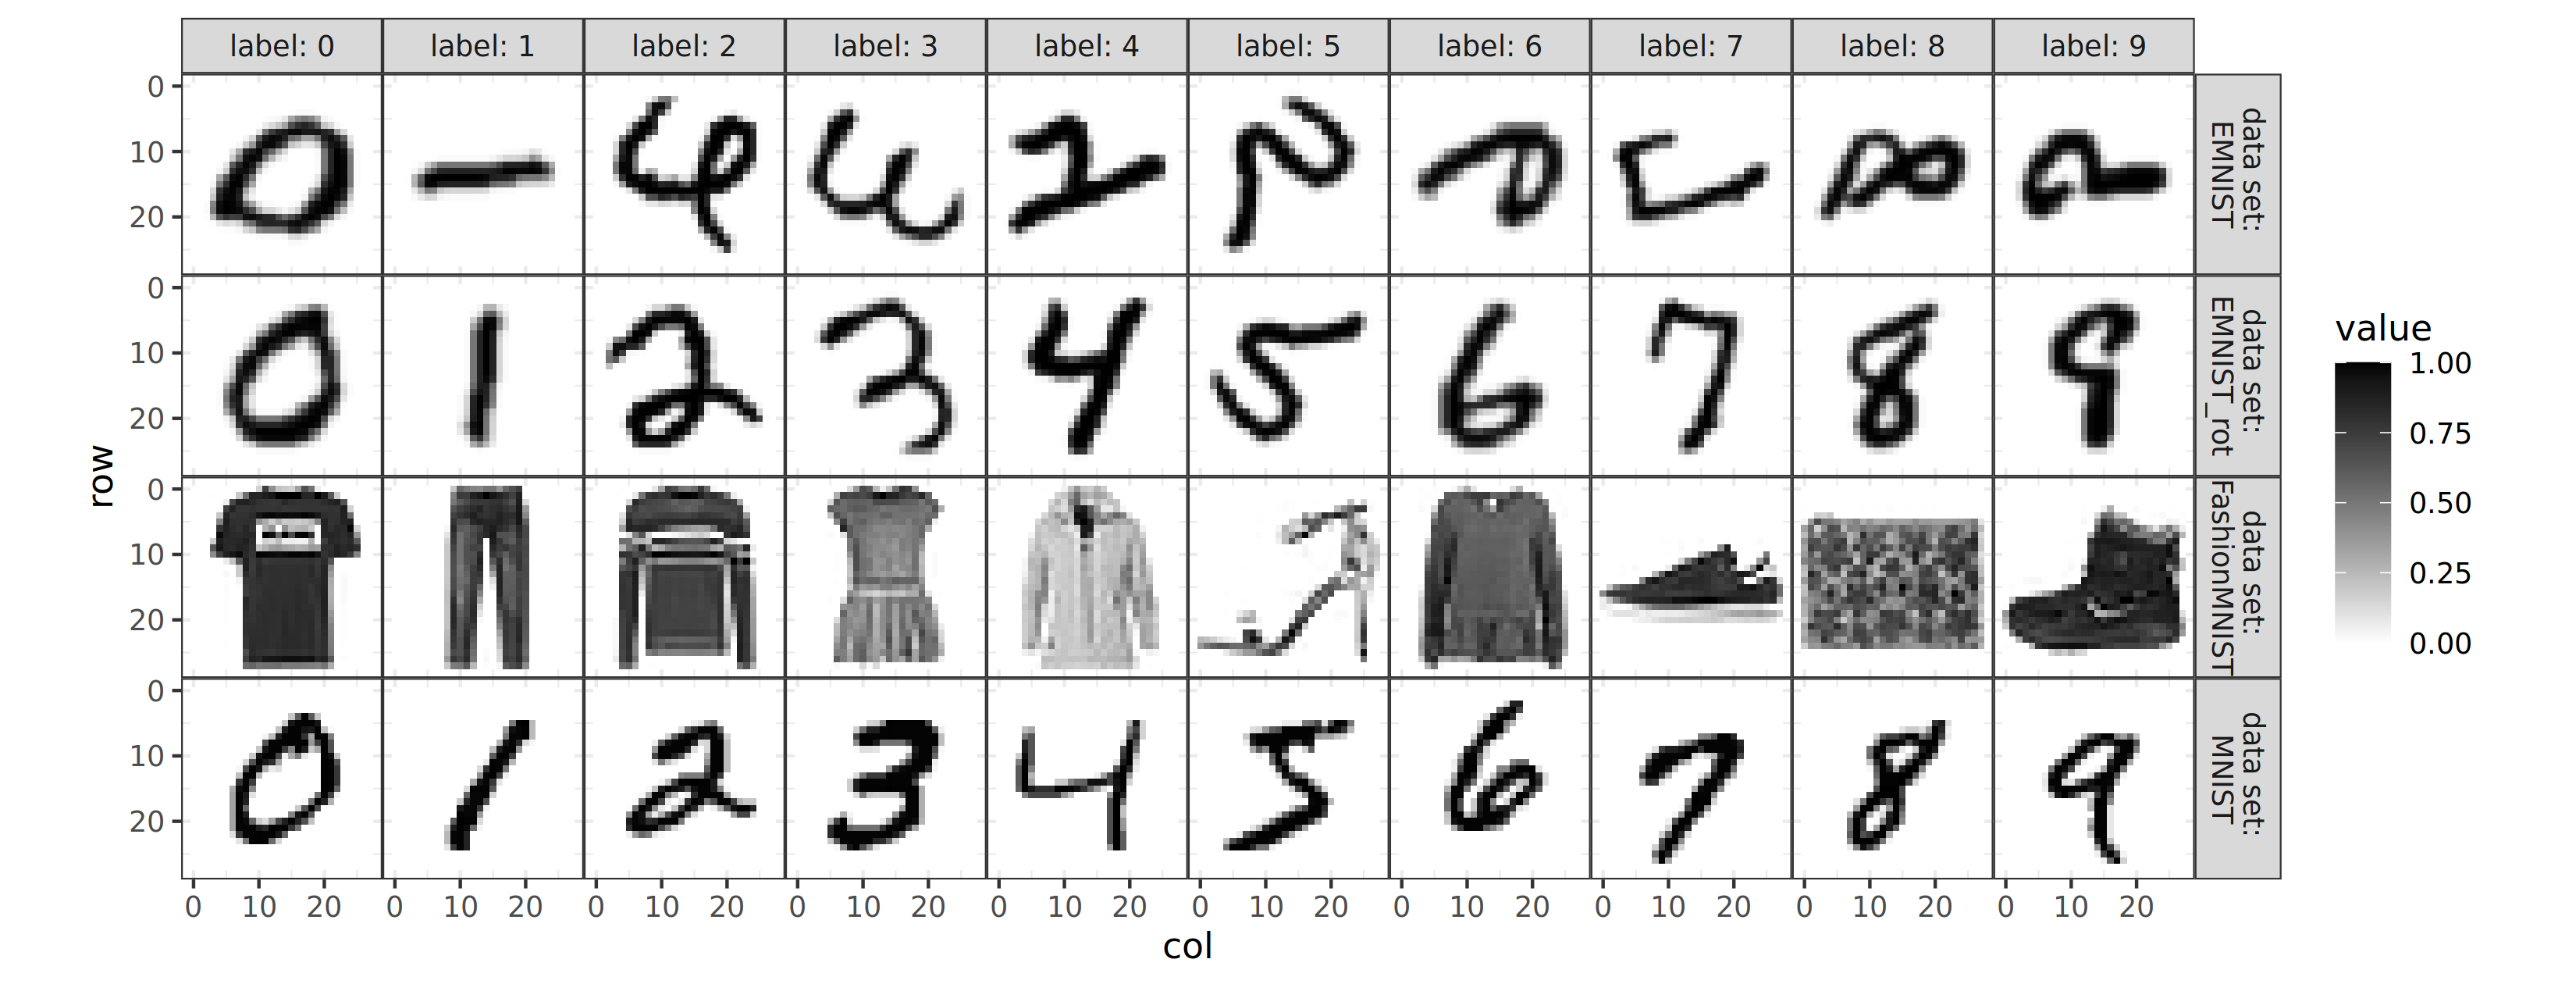
\includegraphics[width=\textwidth]{data_Classif_MNIST_other_1.png}
\end{frame}

\begin{frame}
  \frametitle{Same Other CV for MNIST+FashionMNIST data}

  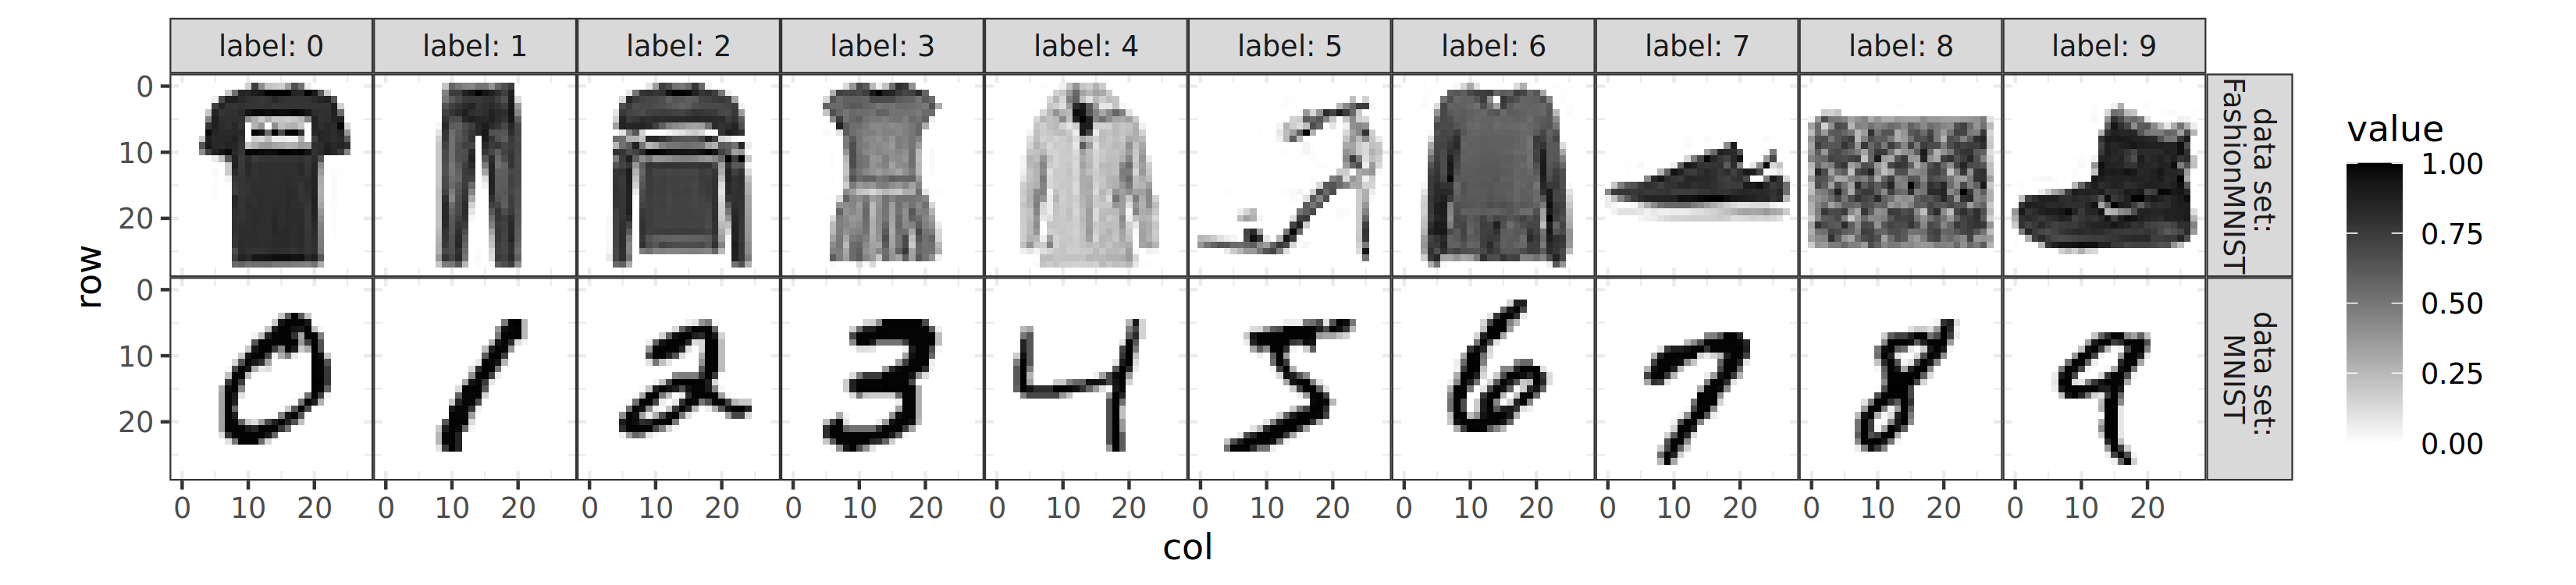
\includegraphics[width=\textwidth]{data_Classif_MNIST_other_FashionMNIST.png}
  
  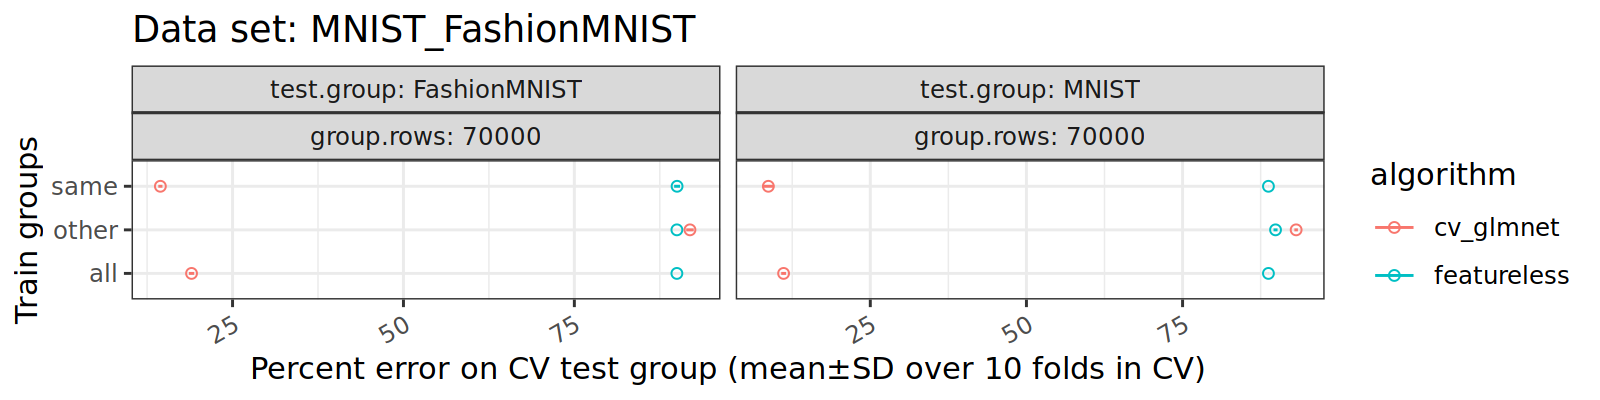
\includegraphics[width=\textwidth]{MNIST_FashionMNIST_error_glmnet_featureless_mean_SD.png}
  \begin{itemize}
  \item Other linear model has more test error than featureless, which
    indicates that the patterns are too different to learn anything at
    all.
  \end{itemize}
\end{frame}

\begin{frame}
  \frametitle{Same Other CV for MNIST+EMNIST data}

  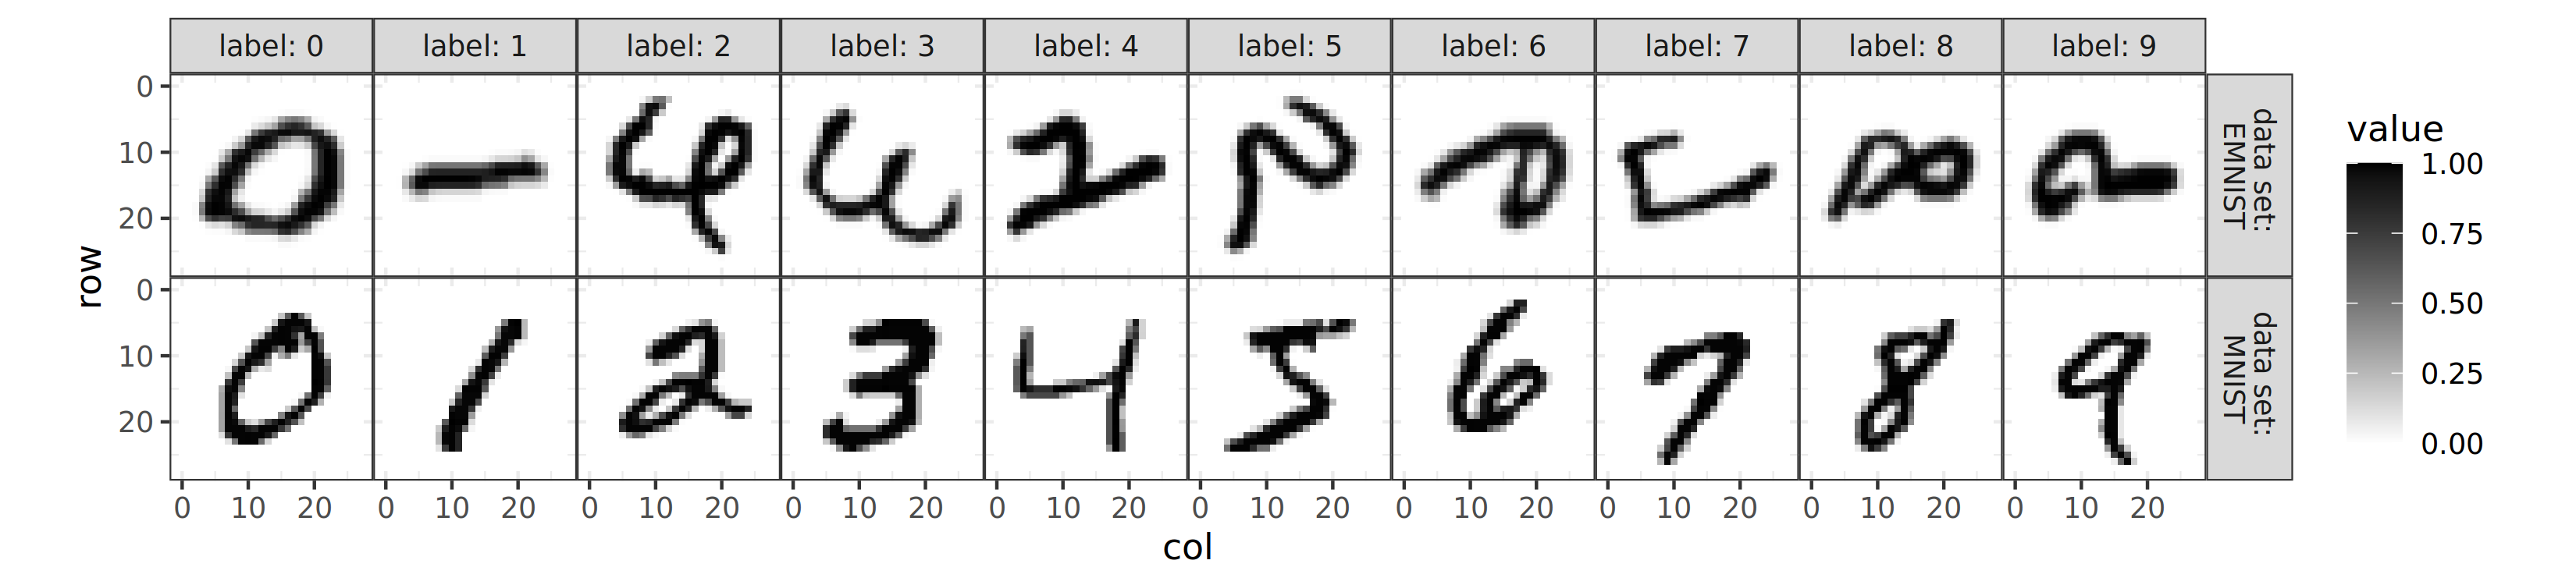
\includegraphics[width=\textwidth]{data_Classif_MNIST_other_EMNIST.png}
  
  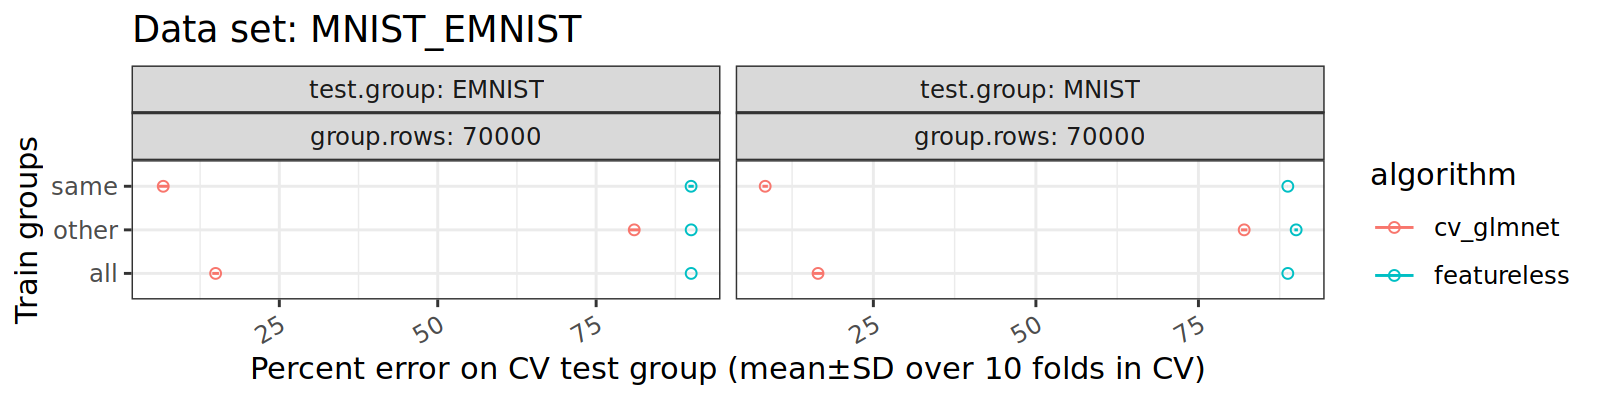
\includegraphics[width=\textwidth]{MNIST_EMNIST_error_glmnet_featureless_mean_SD.png}
  \begin{itemize}
  \item Other has somewhat smaller test error than featureless, so
    something is learned/transferable between data sets, but it is
    still clear that the pattern is very different.
  \end{itemize}
\end{frame}

\begin{frame}
  \frametitle{Same Other CV for MNIST+EMNIST\_rot data}

  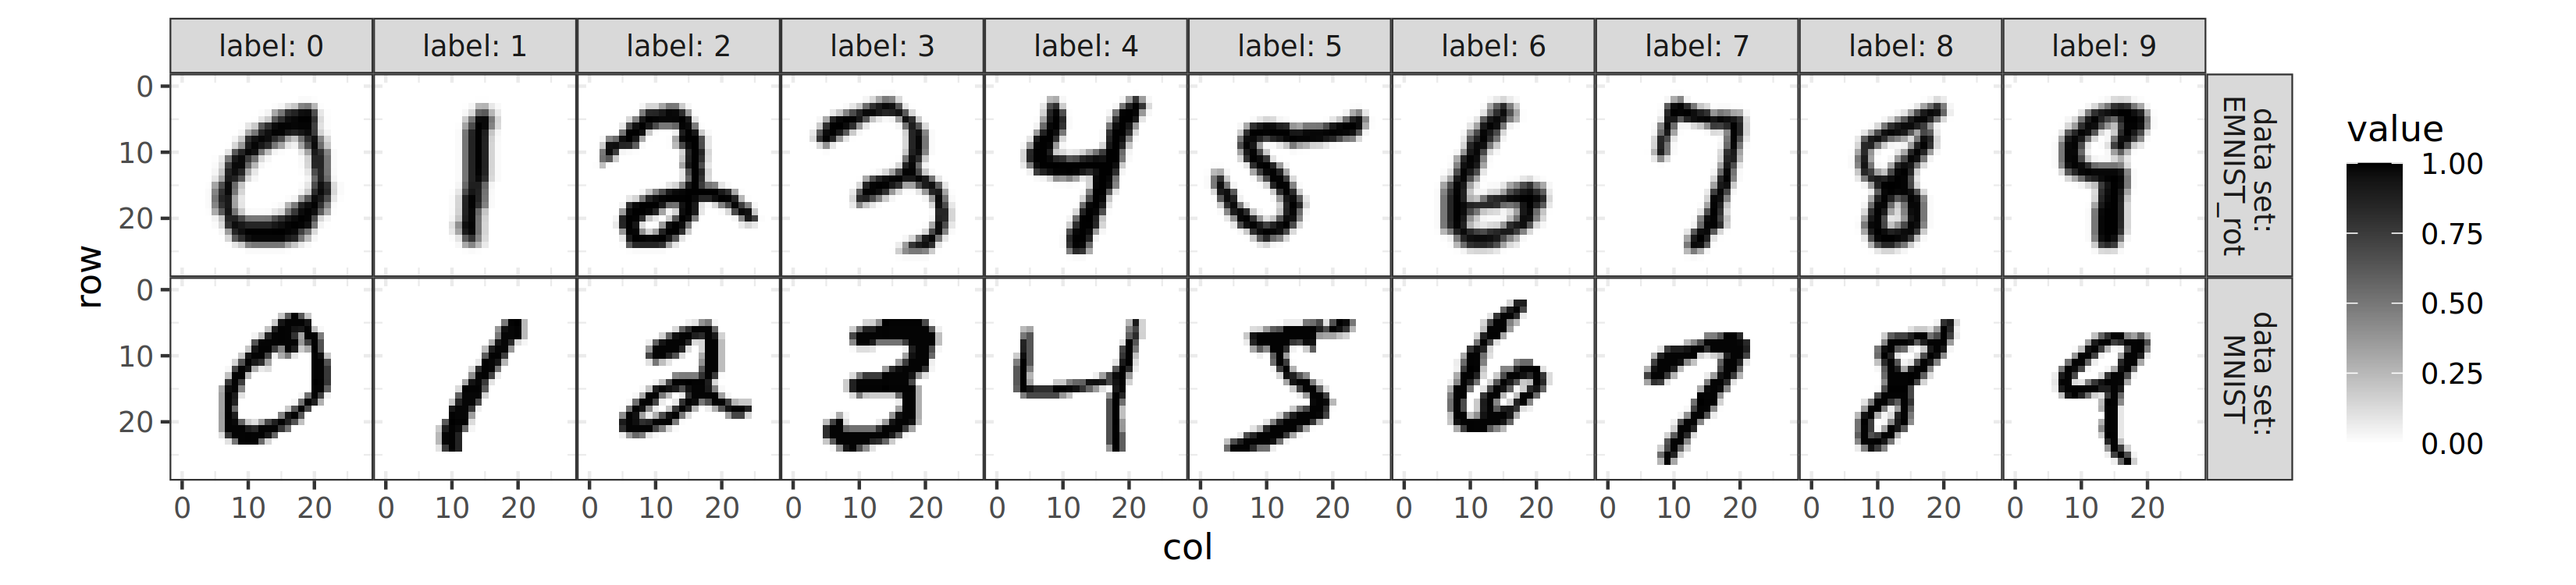
\includegraphics[width=\textwidth]{data_Classif_MNIST_other_EMNIST_rot.png}
  
  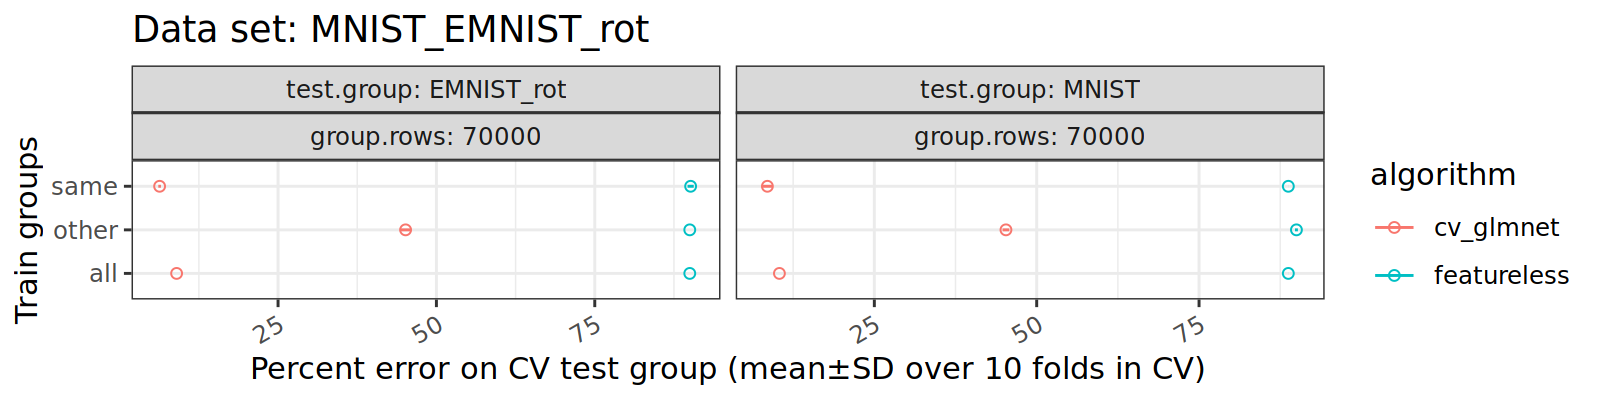
\includegraphics[width=\textwidth]{MNIST_EMNIST_rot_error_glmnet_featureless_mean_SD.png}
  \begin{itemize}
  \item Other still has larger test error than same, indicating some
    similarity between MNIST and EMNIST\_rot data sets.
  \end{itemize}
\end{frame}

\begin{frame}
  \frametitle{Machine learning benchmark data sets}
  \begin{itemize}
  \item Machine learning researchers evaluate new algorithms using
    benchmark data sets, which sometimes have pre-defined train/test
    splits.
% > meta.dt[data.name=="MNIST"]
%    data.name memory.kb  rows n.groups              group.tab group.small.name
%       <char>     <int> <int>    <int>                 <char>           <char>
% 1:     MNIST    429712 70000        2 test=10000;train=60000             test
%    group.small.N group.large.name group.large.N label.small.name label.small.N
%            <int>           <char>         <int>           <char>         <int>
% 1:         10000            train         60000                0          6903
%    label.large.name label.large.N features classes min.rows  test train test%
%              <char>         <int>    <int>   <int>    <int> <int> <int> <int>
% 1:                9          6958      784      10      892 10000 60000    14 
  \item For example MNIST is a data set of images of handwritten
    digits (want to predict which digit, 0 to 9), with 60,000 train
    and 10,000 test images.
% > meta.dt[data.name=="spam"]
%    data.name memory.kb  rows n.groups            group.tab group.small.name
%       <char>     <int> <int>    <int>               <char>           <char>
% 1:      spam      2078  4601        2 test=1536;train=3065             test
%    group.small.N group.large.name group.large.N label.small.name label.small.N
%            <int>           <char>         <int>           <char>         <int>
% 1:          1536            train          3065                0          2788
%    label.large.name label.large.N features classes min.rows  test train test%
%              <char>         <int>    <int>   <int>    <int> <int> <int> <int>
% 1:                1          1813       57       2      595  1536  3065    33
  \item spam is a data set of emails (want to predict spam or not,
    binary), with 3065 train and 1536 test emails.
  \item Are the patterns in the pre-defined train/test sets similar/iid? 
  \item Or are they different? 
  \end{itemize}
\end{frame}

\begin{frame}[fragile]
  \frametitle{Same Other CV for MNIST data (example 1)}
  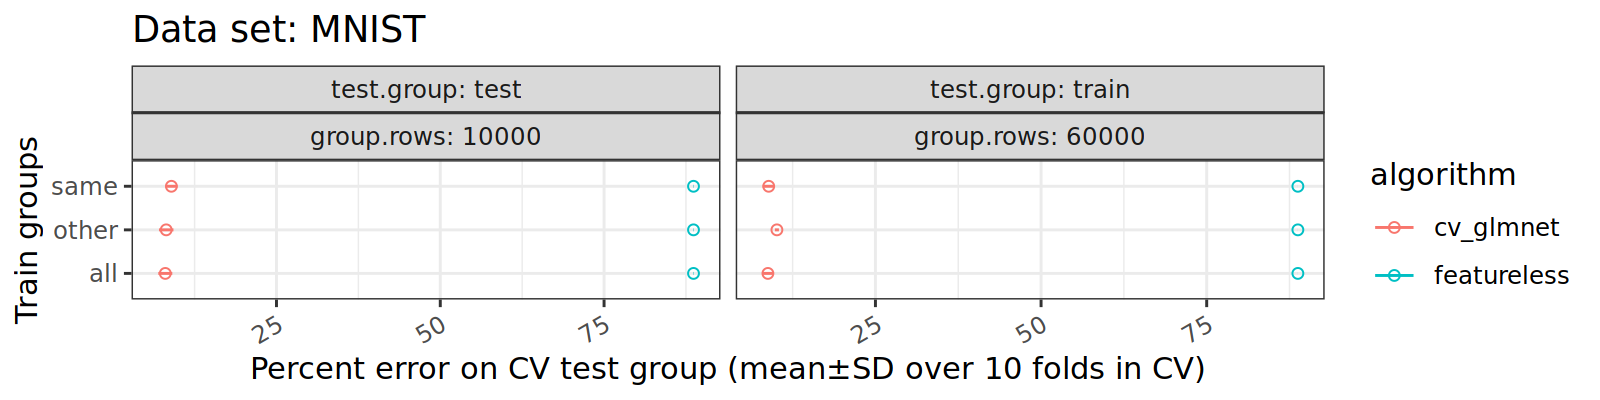
\includegraphics[width=\textwidth]{MNIST_error_glmnet_featureless_mean_SD.png}
  \begin{itemize}
  \item MNIST data are images of handwritten digits (10 classes).
  \item Each linear model has much less error than featureless.
  \end{itemize}
\end{frame}

\begin{frame}
  \frametitle{Same Other CV for MNIST data (example 1)}
  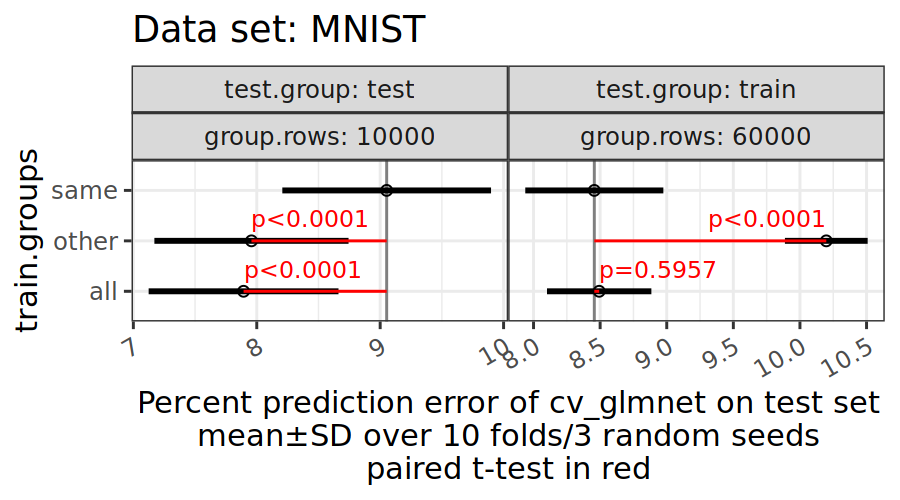
\includegraphics[width=\textwidth]{MNIST_error_glmnet_sizes_mean_SD_pvalue.png}
  \begin{itemize}
  \item When predicting on predefined test set, all has significantly
    lower test error than same, so it is beneficial to combine data
    (similar pattern, not enough data in small test set).
  \end{itemize}
\end{frame}

\begin{frame}[fragile]
  \frametitle{Same Other CV for spam data (example 2)}
  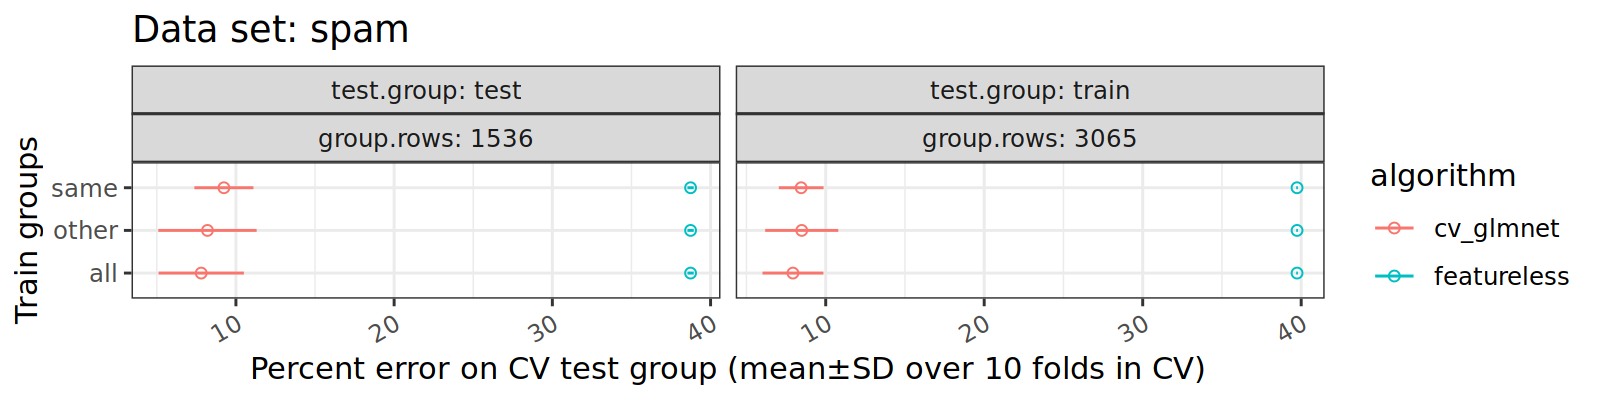
\includegraphics[width=\textwidth]{spam_error_glmnet_featureless_mean_SD.png}
  \begin{itemize}
  \item spam data are emails (binary classification).
  \item Each linear model has much less error than featureless.
  \end{itemize}
\end{frame}

\begin{frame}
  \frametitle{Same Other CV for spam data (example 2)}
  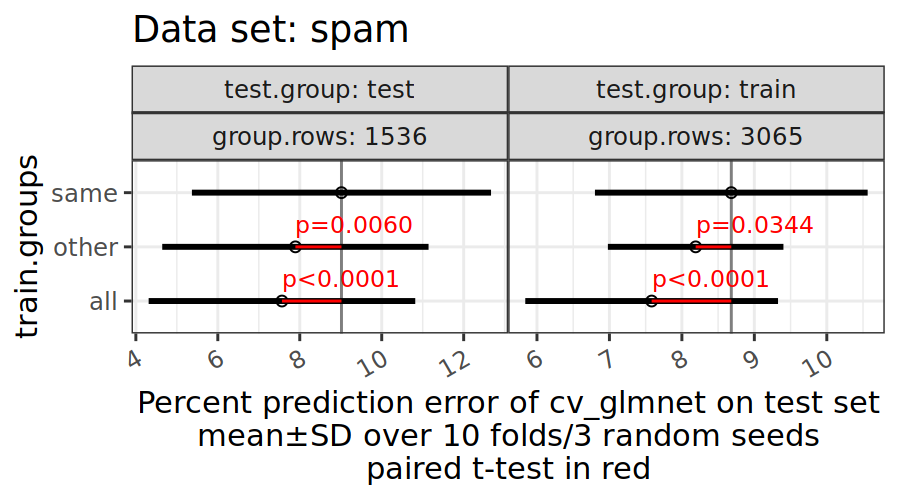
\includegraphics[width=\textwidth]{spam_error_glmnet_sizes_mean_SD_pvalue.png}
  \begin{itemize}
  \item train.groups=all has significantly
    lower test error than same, so it is beneficial to combine data
    (similar pattern, not enough data in either predefined set).
  \end{itemize}
\end{frame}

\begin{frame}[fragile]
  \frametitle{Same Other CV for vowel data (example 3)}
  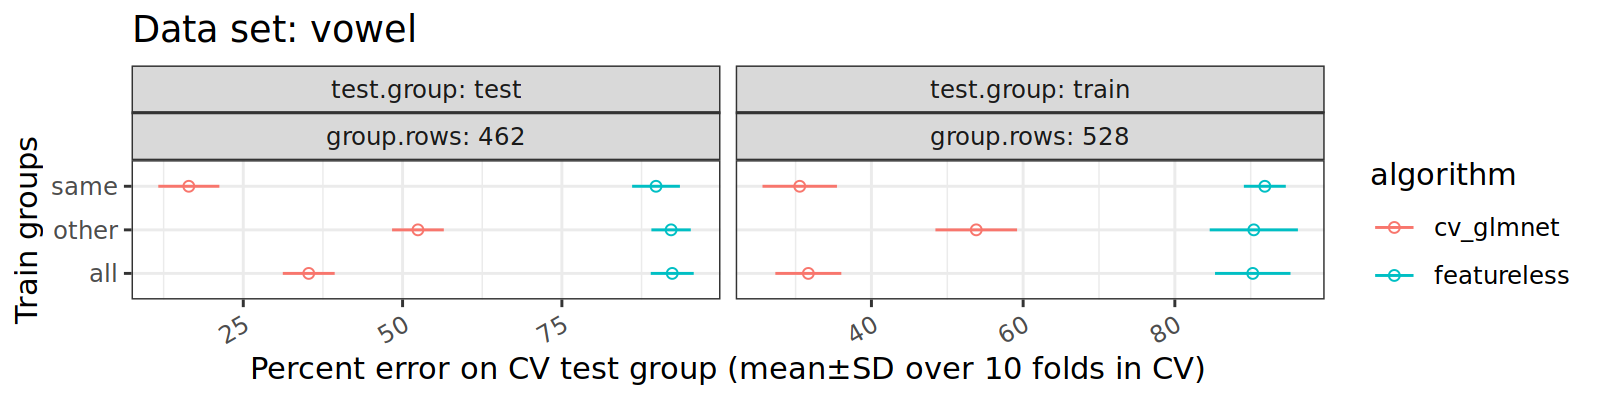
\includegraphics[width=\textwidth]{vowel_error_glmnet_featureless_mean_SD.png}
  \begin{itemize}
%    data.name memory.kb  rows n.groups          group.tab group.small.name
%       <char>     <int> <int>    <int>             <char>           <char>
% 1:     vowel        92   990        2 test=462;train=528             test
%    group.small.N group.large.name group.large.N label.small.name label.small.N
%            <int>           <char>         <int>           <char>         <int>
% 1:           462            train           528                1            90
%    label.large.name label.large.N features classes min.rows  test train test%
%              <char>         <int>    <int>   <int>    <int> <int> <int> <int>
% 1:               11            90       10      11       42   462   528    46
  \item vowel data are audio/speech recordings (11 classes/speakers).
  \item Each linear model has much less error than featureless.
  \end{itemize}
\end{frame}

\begin{frame}
  \frametitle{Same Other CV for vowel data (example 3)}
  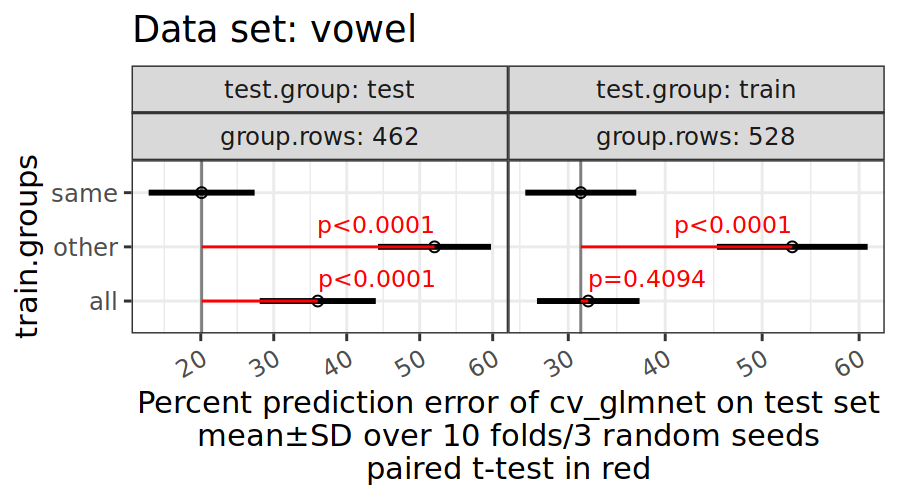
\includegraphics[width=\textwidth]{vowel_error_glmnet_sizes_mean_SD_pvalue.png}
  \begin{itemize}
  \item train.groups=all has significantly larger test error than
    same, indicating that it is not optimal to combine the
    predefined sets (which have different patterns). 
  \end{itemize}
\end{frame}

\begin{frame}[fragile]
  \frametitle{Same Other CV for KMNIST data (example 4)}
  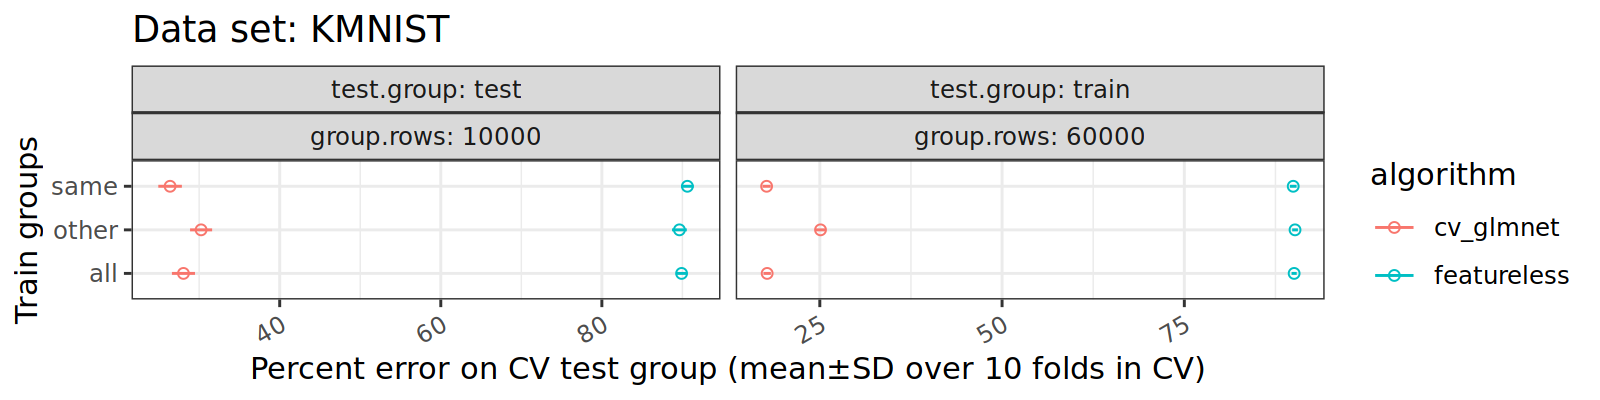
\includegraphics[width=\textwidth]{KMNIST_error_glmnet_featureless_mean_SD.png}
  \begin{itemize}
  \item KMNIST are images of handwritten Japanese (10 classes).
  \item Each linear model has much less error than featureless.
  \end{itemize}
\end{frame}

\begin{frame}
  \frametitle{Same Other CV for KMNIST data (example 4)}
  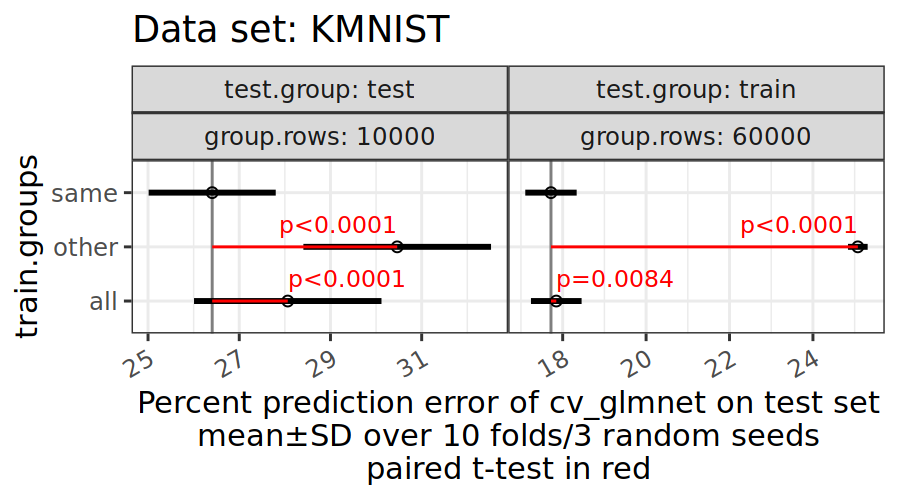
\includegraphics[width=\textwidth]{KMNIST_error_glmnet_sizes_mean_SD_pvalue.png}
  \begin{itemize}
  \item train.groups=all has significantly larger test error than
    same, indicating that it is not optimal to combine the
    predefined sets (which have different patterns). 
  \end{itemize}
\end{frame}

\section{Synthesis, Discussion and Conclusions}

\begin{frame}
  \frametitle{A spectrum of similarity and differences}
  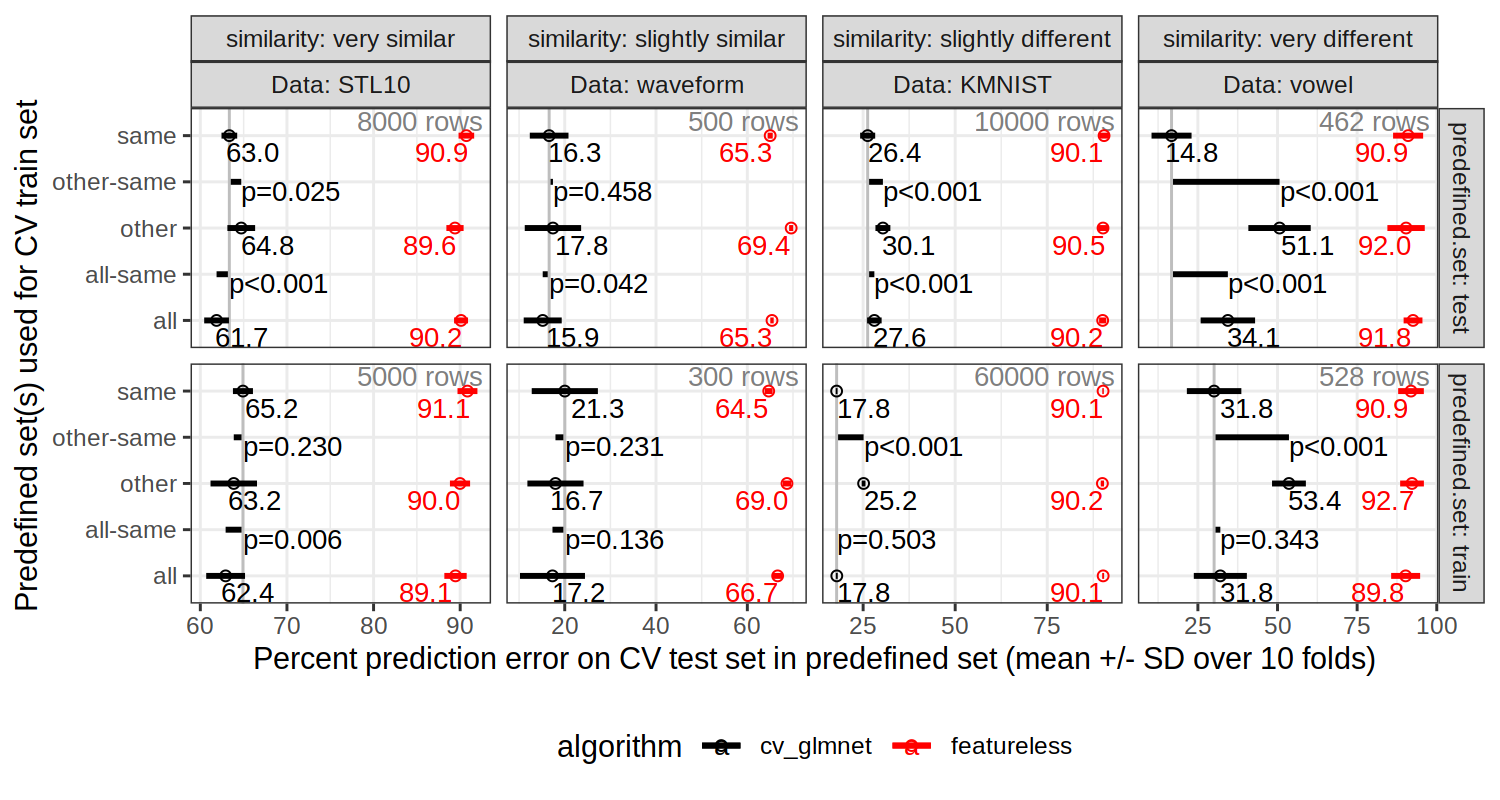
\includegraphics[width=\textwidth]{data_Classif_batchmark_registry_glmnet_featureless_mean_sd}
  \begin{itemize}
  \item Different patterns of same/other/all
    test error rates, depending on the similarity of the
    groups in each data set.
  \end{itemize}
\end{frame}
 
\begin{frame}
  \frametitle{Data sets analyzed}
  \begin{itemize}
  \item Sorted by test error difference between all and same.
  \item Different groups on top/positive.
  \item Similar groups on bottom/negative.
  \end{itemize}
  \scriptsize
\begin{tabular}{rlrrrrr}
  \hline
 & data.name & rows & features & classes & n.groups & all-same \\ 
  \hline
1 & vowel & 990 &  10 &  11 &   2 & 9.98 \\ 
  2 & CanadaFires\_downSampled & 1491 &  46 &   2 &   4 & 4.02 \\ 
  3 & CanadaFires\_all & 4827 &  46 &   2 &   4 & 3.39 \\ 
  4 & aztrees4 & 5956 &  21 &   2 &   4 & 2.28 \\ 
  5 & aztrees3 & 5956 &  21 &   2 &   3 & 2.05 \\ 
  6 & FishSonar\_river & 2815744 &  81 &   2 &   4 & 1.69 \\ 
  7 & KMNIST & 70000 & 784 &  10 &   2 & 0.87 \\
  \hline
  8 & NSCH\_autism & 46010 & 364 &   2 &   2 & -0.03 \\ 
  9 & MNIST & 70000 & 784 &  10 &   2 & -0.53 \\ 
  10 & QMNIST & 120000 & 784 &  10 &   2 & -0.70 \\ 
  11 & spam & 4601 &  57 &   2 &   2 & -0.77 \\ 
  12 & EMNIST & 70000 & 784 &  10 &   2 & -0.85 \\ 
  13 & FashionMNIST & 70000 & 784 &  10 &   2 & -0.97 \\ 
  14 & zipUSPS & 9298 & 256 &  10 &   2 & -1.44 \\ 
  15 & waveform & 800 &  21 &   3 &   2 & -1.54 \\ 
  16 & CIFAR10 & 60000 & 3072 &  10 &   2 & -1.77 \\ 
  17 & STL10 & 13000 & 27648 &  10 &   2 & -1.97 \\ 
   \hline
\end{tabular}

\end{frame}

\begin{frame}
  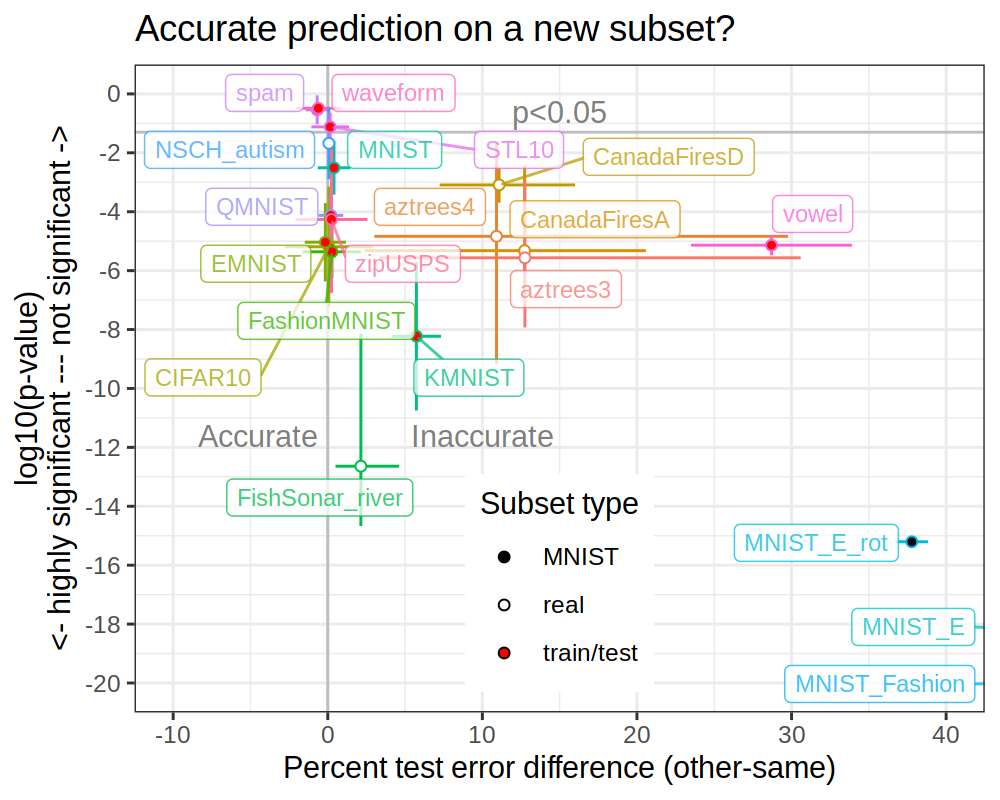
\includegraphics[height=\textheight]{data_Classif_batchmark_registry_scatter_other_segments.png} 
\end{frame}

\begin{frame}
  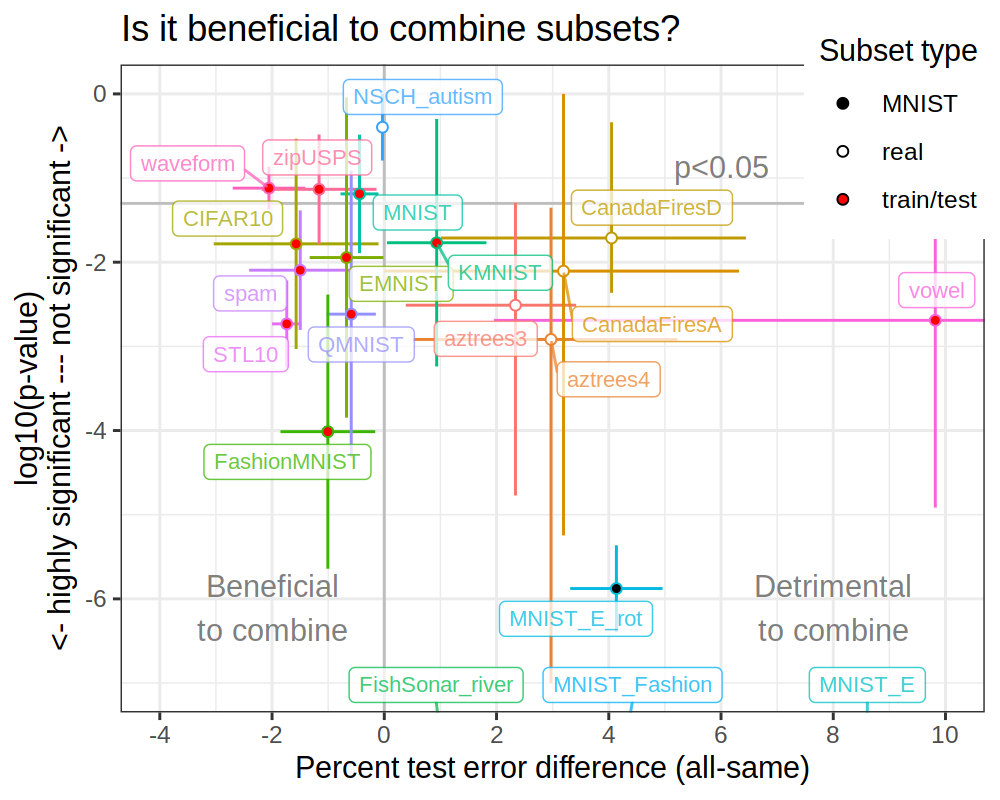
\includegraphics[height=\textheight]{data_Classif_batchmark_registry_scatter_all_segments.png}
\end{frame}
 
\begin{frame}
  \frametitle{Discussion and Conclusions}
  \begin{itemize}
  \item Proposed Same Other Cross-Validation shows if
    data sets are similar enough to so that combining data is
    beneficial for learning (train on one group, test/predict on
    another).
  \item In Autism data, there was a slight benefit to combining years.
  \item In fires/trees/fish data, we observed
    significant differences between images/regions/rivers.
  \item Some pre-defined train/test splits in benchmark data sets
    are similar/iid (MNIST/spam), others are not (KMNIST/vowel).
  \item Free/open-source R package available:
    \url{https://github.com/tdhock/mlr3resampling}
  \item These slides are reproducible, using the code in \url{https://github.com/tdhock/cv-same-other-paper}
  \item Contact: toby.hocking@nau.edu,
    toby.hocking@r-project.org
  \end{itemize}
\end{frame}

\section{Supplementary slides}

\begin{frame}
  \frametitle{Same Other CV for Autism data}
  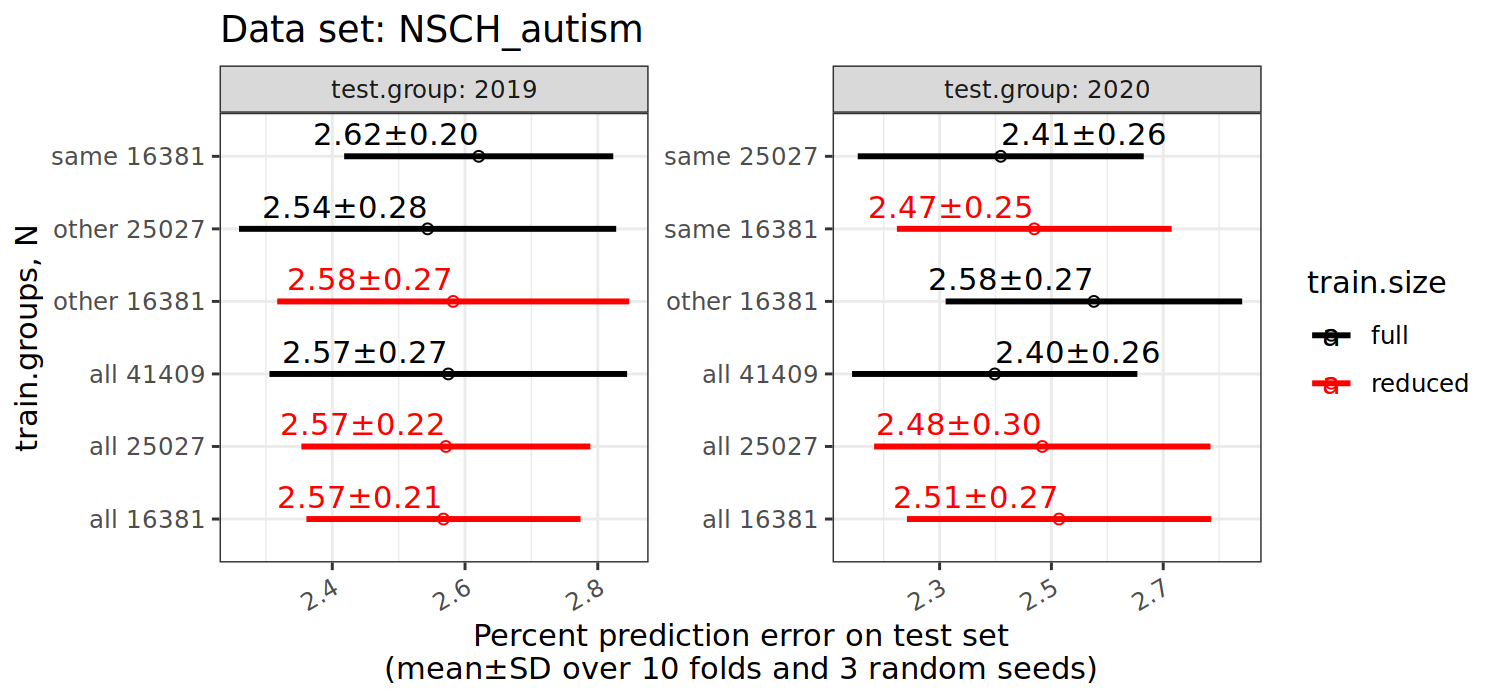
\includegraphics[width=\textwidth]{NSCH_autism_error_glmnet_sizes_mean_sd_more.png}
  \begin{itemize}
  \item Reduced sizes (red) are used to judge the effect of sample size.
  \item Sample size effect present for test group 2020, but not 2019.
  \end{itemize}
\end{frame}

\begin{frame}
  \frametitle{Same Other CV for Canada fires data}
  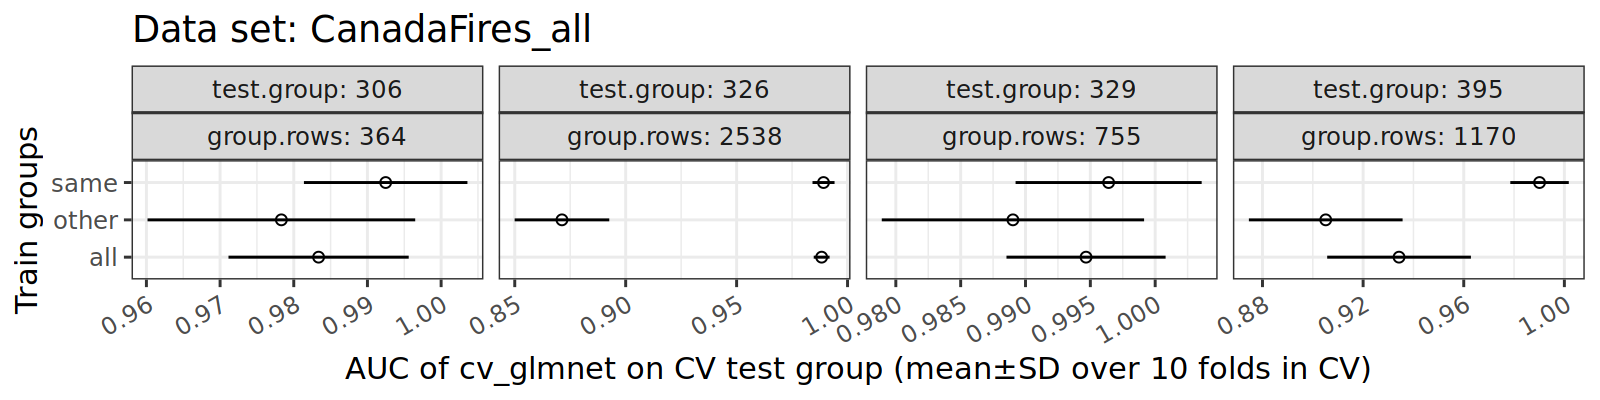
\includegraphics[width=\textwidth]{CanadaFires_all_AUC_glmnet_mean_SD.png}
  \begin{itemize}
  \item Area Under the ROC Curve (AUC) is a good measure of accuracy
    for imbalanced binary classification problems (constant/featureless=0.5, best=1).
  \item Test AUC for all is never as large as same, indicating that
    you need data from the same river for optimal prediction accuracy.
  \end{itemize}
\end{frame}

\begin{frame}
  \frametitle{Same Other CV for AZ trees data}
  \includegraphics[width=\textwidth]{AZtrees3_AUC_glmnet_mean_SD.png}
  \begin{itemize}
  \item Area Under the ROC Curve (AUC) is a good measure of accuracy
    for imbalanced binary classification problems (constant/featureless=0.5, best=1).
  \item Test AUC for all is never as large as same, indicating that
    you need data from the same river for optimal prediction accuracy.
  \end{itemize}
\end{frame}

\begin{frame}[fragile]
  \frametitle{Same Other CV for STL10 data}
  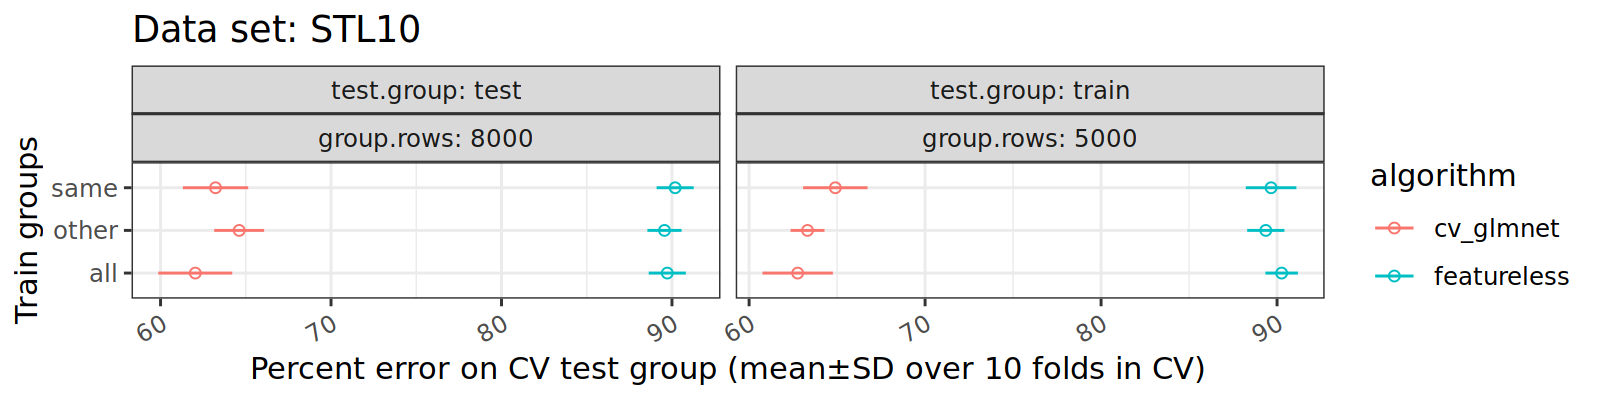
\includegraphics[width=\textwidth]{STL10_error_glmnet_featureless_mean_SD.png}
  \begin{itemize}
  \item Image classification data (10 different objects).
  \item Each linear model has much less error than featureless.
  \end{itemize}
\end{frame}

\begin{frame}
  \frametitle{Same Other CV for STL10 data}
  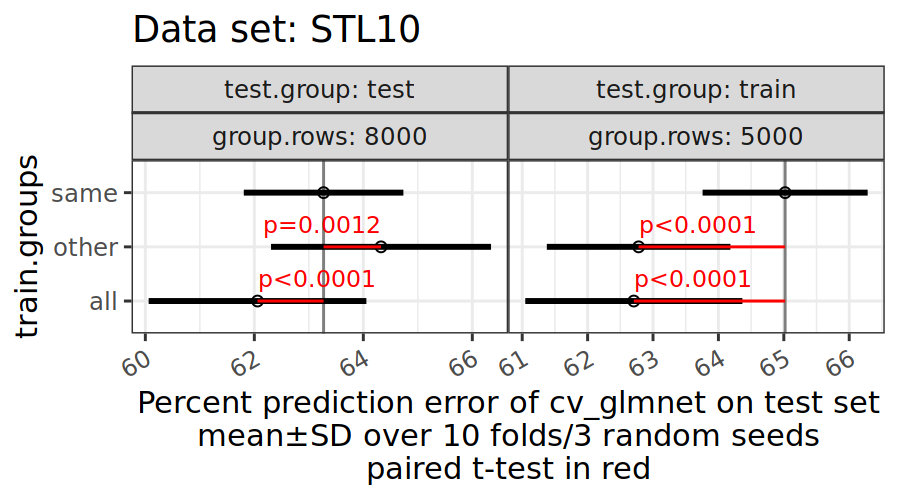
\includegraphics[width=\textwidth]{STL10_error_glmnet_sizes_mean_SD_pvalue.png}
  \begin{itemize}
  \item train.groups=all has significantly
    lower test error than same, so it is beneficial to combine data
    (similar pattern, not enough data in predefined train set).
  \end{itemize}
\end{frame}

\begin{frame}[fragile]
  \frametitle{Same Other CV for CIFAR10 data}
  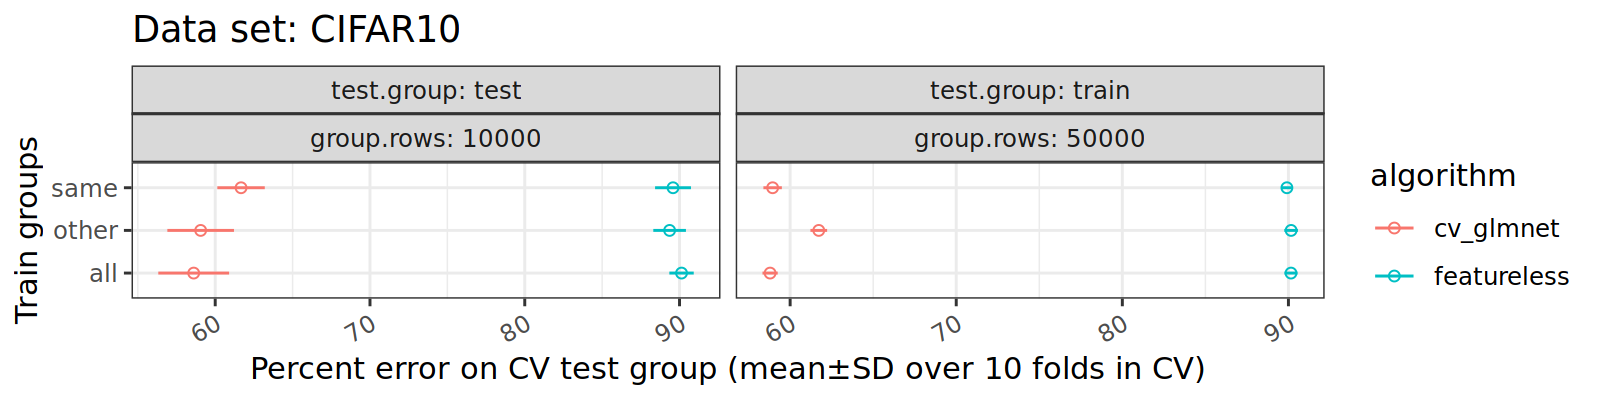
\includegraphics[width=\textwidth]{CIFAR10_error_glmnet_featureless_mean_SD.png}
  \begin{itemize}
  \item Image classification data (10 different objects).
  \item Each linear model has much less error than featureless.
  \end{itemize}
\end{frame}

\begin{frame}
  \frametitle{Same Other CV for CIFAR10 data}
  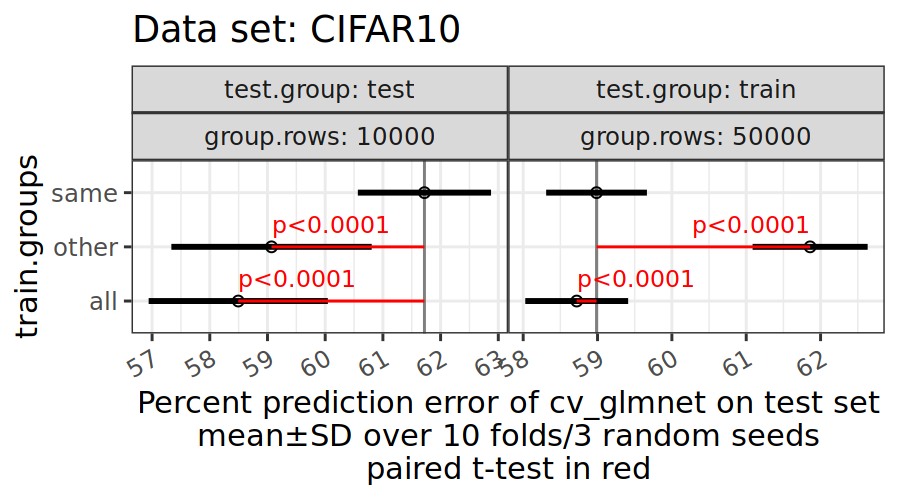
\includegraphics[width=\textwidth]{CIFAR10_error_glmnet_sizes_mean_SD_pvalue.png}
  \begin{itemize}
  \item train.groups=all has significantly
    lower test error than same, so it is beneficial to combine data
    (similar pattern, not enough data in predefined test set).
  \end{itemize}
\end{frame}

\end{document}
